% lecture8_ro.tex -- GENERATED by build_L8.py from L8_numbers.json; do not edit by hand.
\documentclass[10pt,aspectratio=169,t]{beamer}
% =============================================================================
% nn_preamble.tex -- shared Beamer preamble of Neural Networks and Deep Learning (NN)
% Used by every lecture: lectures/Lk/lecturek.tex does
%   \documentclass[10pt,aspectratio=169,t]{beamer}
%   % =============================================================================
% nn_preamble.tex -- shared Beamer preamble of Neural Networks and Deep Learning (NN)
% Used by every lecture: lectures/Lk/lecturek.tex does
%   \documentclass[10pt,aspectratio=169,t]{beamer}
%   % =============================================================================
% nn_preamble.tex -- shared Beamer preamble of Neural Networks and Deep Learning (NN)
% Used by every lecture: lectures/Lk/lecturek.tex does
%   \documentclass[10pt,aspectratio=169,t]{beamer}
%   \input{../common/nn_preamble}
%   \nnlecture{k}{Lecture title}
% Logos live in lectures/common/logos/, charts in lectures/Lk/charts/.
% Do NOT add \hfuzz / \vfuzz / \hbadness here: overfull boxes must be fixed, not hidden.
% =============================================================================

\usetheme{default}
\setbeamersize{text margin left=7mm, text margin right=7mm}

% ---------------------------------------------------------------- packages
\usepackage[utf8]{inputenc}
\usepackage[T1]{fontenc}
\usepackage{lmodern}
\usepackage{amsmath, amssymb}
\usepackage{mathtools}
\usepackage{bm}
\usepackage{tikz}
\usetikzlibrary{arrows.meta, positioning, calc, shapes.misc}
\usepackage{booktabs}
\usepackage{array}
\usepackage{graphicx}
\usepackage{colortbl}
\usepackage{xcolor}
\usepackage{multicol}
\hypersetup{colorlinks=true, linkcolor=MainBlue, urlcolor=MainBlue, citecolor=MainBlue}
\graphicspath{{../common/logos/}}   % charts are included with their language folder: charts/en/, charts/ro/

% ---------------------------------------------------------------- colours
\definecolor{MainBlue}{RGB}{26, 58, 110}
\definecolor{IDAred}{RGB}{205, 0, 0}
\definecolor{DarkGray}{RGB}{51, 51, 51}
\definecolor{FooterGray}{RGB}{100, 100, 100}
\definecolor{BlockGray}{RGB}{236, 238, 242}
\definecolor{KeynoteGray}{RGB}{218, 218, 218}
\definecolor{Crimson}{RGB}{190, 40, 50}
\definecolor{Forest}{RGB}{30, 110, 50}
\definecolor{Bitter}{RGB}{214, 150, 20}
% chart palette (same hex values and order as lectures/common/nn_plot.py SERIES)
\definecolor{Ser1}{HTML}{2A78D6}
\definecolor{Ser2}{HTML}{EB6834}
\definecolor{Ser3}{HTML}{1BAF7A}
\definecolor{Ser4}{HTML}{EDA100}
\definecolor{Ser5}{HTML}{E87BA4}
\definecolor{Ser6}{HTML}{008300}
\definecolor{Ser7}{HTML}{6250D6}
\definecolor{Ser8}{HTML}{E34948}

\setbeamertemplate{background}{%
  \begin{tikzpicture}[remember picture, overlay]
    \shade[shading=axis, shading angle=315, top color=white, bottom color=KeynoteGray]
      (current page.south west) rectangle (current page.north east);
  \end{tikzpicture}}
\setbeamercolor{background canvas}{bg=}
\setbeamercolor{structure}{fg=MainBlue}
\setbeamercolor{normal text}{fg=DarkGray}
\setbeamercolor{title}{fg=IDAred}
\setbeamercolor{frametitle}{fg=IDAred, bg=}
\setbeamercolor{block title}{bg=MainBlue, fg=white}
\setbeamercolor{block body}{bg=BlockGray, fg=DarkGray}
\setbeamercolor{block title alerted}{bg=Crimson, fg=white}
\setbeamercolor{block body alerted}{bg=Crimson!7, fg=DarkGray}
\setbeamercolor{block title example}{bg=Forest, fg=white}
\setbeamercolor{block body example}{bg=Forest!7, fg=DarkGray}
\setbeamercolor{item}{fg=MainBlue}
\setbeamerfont{frametitle}{size=\large, series=\bfseries}
\setbeamerfont{block title}{size=\small, series=\bfseries}
\setbeamertemplate{blocks}[rounded][shadow=false]
\setbeamertemplate{itemize item}{\color{MainBlue}$\boxdot$}
\setbeamertemplate{itemize subitem}{\color{MainBlue}\scriptsize$\blacktriangleright$}
% compact two-level lists: level 1 = main point, level 2 = details (no text outside bullets)
\setbeamerfont{itemize/enumerate subbody}{size=\footnotesize}
\setlength{\leftmargini}{1.1em}
\setlength{\leftmarginii}{1.1em}
\setbeamertemplate{itemize/enumerate body begin}{\setlength{\topsep}{0pt}\setlength{\partopsep}{0pt}\setlength{\parskip}{0pt}}
\setbeamertemplate{itemize/enumerate subbody begin}{\setlength{\topsep}{0pt}\setlength{\partopsep}{0pt}\setlength{\itemsep}{0pt}\vspace{-0.4ex}}

\setbeamertemplate{enumerate item}{\color{MainBlue}\insertenumlabel.}
\setlength{\leftmargini}{1.3em}
\setlength{\leftmarginii}{1.2em}
\setbeamertemplate{navigation symbols}{}
\setbeamertemplate{section in toc}{\color{MainBlue}$\blacktriangleright$~\inserttocsection}
\setbeamertemplate{caption}{\raggedright\insertcaption\par}
% frame subtitle = precise citation line under the claim title (Weron style)
\setbeamerfont{framesubtitle}{size=\footnotesize}
\setbeamercolor{framesubtitle}{fg=FooterGray}
% outline that reappears at every section with the current section highlighted
\setbeamertemplate{section in toc shaded}[default][35]
\setbeamertemplate{subsection in toc shaded}[default][35]
\setbeamertemplate{subsection in toc}{\leavevmode\leftskip=2.2em\color{DarkGray}\small\inserttocsubsection\par}
\AtBeginSection[]{{\begin{frame}{\txtoutline}\vspace{2mm}\small
  \tableofcontents[currentsection,hideothersubsections]\end{frame}}}

% ---------------------------------------------------------------- head and foot
\setbeamertemplate{headline}{%
  \vskip10pt%
  \hbox to \paperwidth{\hskip0.5cm%
    {\small\color{FooterGray}\renewcommand{\hyperlink}[2]{##2}\insertsectionhead}%
    \hfill\textcolor{FooterGray}{\small\insertframenumber}\hskip0.5cm}%
  \vskip4pt{\color{FooterGray}\hrule height 0.4pt}}
% footer as in the other courses (MFM, SFM): course name on the left, small sparkline on the right
\setbeamertemplate{footline}{%
  {\color{FooterGray}\hrule height 0.4pt}\vskip4pt%
  \hbox to \paperwidth{\hskip0.5cm%
    \textcolor{FooterGray}{\small\txtcourse}%
    \hfill\raisebox{-0.1em}{\begin{tikzpicture}[x=0.08em, y=0.08em, line width=0.4pt]
      \draw[FooterGray] (0,3) -- (1,4) -- (2,3.5) -- (3,5) -- (4,4) -- (5,6) -- (6,5.5) -- (7,4) -- (8,5) -- (9,7) -- (10,6) -- (11,5) -- (12,6.5) -- (13,8) -- (14,7) -- (15,6) -- (16,7.5) -- (17,9) -- (18,8) -- (19,7) -- (20,8.5) -- (21,10) -- (22,9) -- (23,8) -- (24,9.5);
    \end{tikzpicture}}\hskip0.5cm}%
  \vskip6pt}

% ---------------------------------------------------------------- title page
\defbeamertemplate*{title page}{nn}[1][]{%
  \vspace{0.15cm}
  \begin{center}
    \href{https://www.ase.ro}{
\includegraphics[height=0.9cm]{ase_logo.png}}\hspace{0.3cm}%
    \href{https://ipe.ro/new}{
\includegraphics[height=0.9cm]{acad_logo.png}}\hspace{0.3cm}%
    \href{https://theida.net}{
\includegraphics[height=0.9cm]{ida_logo.png}}\hspace{0.3cm}%
    \href{https://blockchain-research-center.com}{
\includegraphics[height=0.9cm]{brc_logo.png}}\hspace{0.3cm}%
    \href{https://www.ai4efin.ase.ro}{
\includegraphics[height=0.9cm]{ai4efin_logo.png}}\hspace{0.3cm}%
    \href{https://www.digital-finance-msca.com}{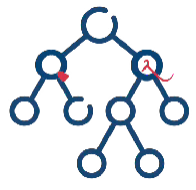
\includegraphics[height=0.9cm]{msca_logo.png}}%
  \end{center}
  \vspace{0.45cm}
  \begin{center}
    \begin{minipage}{0.1\textwidth}\centering
      \href{https://quantlet.com}{
\includegraphics[height=0.9cm]{ql_logo.png}}\end{minipage}%
    \begin{minipage}{0.78\textwidth}\centering
      {\Large\bfseries\usebeamercolor[fg]{title}\inserttitle}\par\vspace{0.25cm}
      {\large\usebeamercolor[fg]{title}\insertsubtitle}\end{minipage}%
    \begin{minipage}{0.1\textwidth}\centering
      \href{https://quantinar.com}{
\includegraphics[height=0.9cm]{qr_logo.png}}\end{minipage}
  \end{center}
  \vfill
  \hspace{0.4cm}{\bfseries\insertauthor}\par\vspace{0.12cm}
  \hspace{0.4cm}\begin{minipage}[t]{0.92\textwidth}\raggedright\footnotesize\insertinstitute\end{minipage}
  \par\vspace{0.4cm}}

% ---------------------------------------------------------------- lecture metadata
\newcommand{\nnshort}{}
\newcommand{\nnnb}{notebooks}
\newcommand{\nnrepo}{https://github.com/danpele/NEURAL_BIZ/tree/main}
% language-dependent labels (English default; \nnromanian switches to Romanian, call it before \nnlecture)
\newcommand{\txtcourse}{Neural Networks and Deep Learning}
\newcommand{\txtlecture}{Lecture}
\newcommand{\txtoutline}{Outline}
\newcommand{\txtintuition}{In one sentence:}
\newcommand{\txtjob}{In practice:}
\newcommand{\txttry}{Experiment yourself:}
\newcommand{\txtwhere}{where}
\newcommand{\txtsim}{SIMULATED DATA (teaching illustration)}
\newcommand{\txtnbsuffix}{}
\newcommand{\txtinstitute}{Bucharest University of Economic Studies (ASE), Department of Statistics and Econometrics\\
    Romanian Academy, Institute for Economic Forecasting (IPE)\\
    IDA Institute Digital Assets \textbullet\ AI4EFin \textbullet\ MSCA Digital Finance}
\newcommand{\nnromanian}{%
  \renewcommand{\txtcourse}{Rețele neuronale și deep learning}%
  \renewcommand{\txtlecture}{Cursul}%
  \renewcommand{\txtoutline}{Cuprins}%
  \renewcommand{\txtintuition}{Pe scurt:}%
  \renewcommand{\txtjob}{În practică:}%
  \renewcommand{\txttry}{Exercițiu practic:}%
  \renewcommand{\txtwhere}{unde}%
  \renewcommand{\txtsim}{DATE SIMULATE (doar pentru ilustrare)}%
  \renewcommand{\txtnbsuffix}{\string_ro}%
  \renewcommand{\txtinstitute}{Academia de Studii Economice din București (ASE), Departamentul de Statistică și Econometrie\\
    Academia Română, Institutul de Prognoză Economică (IPE)\\
    IDA Institute Digital Assets \textbullet\ AI4EFin \textbullet\ MSCA Digital Finance}}
\newcommand{\nnlecture}[2]{%
  \renewcommand{\nnshort}{\txtlecture\ #1}%
  \renewcommand{\nnnb}{notebooks/L#1\string_notebook\txtnbsuffix.ipynb}%
  \title[NN]{\txtcourse}%
  \subtitle{\txtlecture\ #1: #2}%
  \author{Prof.\ dr.\ Daniel Traian PELE}%
  \institute{\txtinstitute}%
  \date{}}

% ---------------------------------------------------------------- teaching blocks (one message per frame)
% \intuition{one plain sentence}  ->  formula with every symbol defined  ->  real-data example  ->  \manager{one line}
\newcommand{\intuition}[1]{\begin{itemize}\item {\color{MainBlue}\textbf{\txtintuition}}~#1\end{itemize}\vspace{0.6mm}}
\newcommand{\manager}[1]{\colorbox{Forest!10}{\parbox{\dimexpr\linewidth-2\fboxsep\relax}{\footnotesize
  \begin{itemize}\setlength{\itemsep}{0pt}\item \textbf{\color{Forest}\txtjob}~#1\end{itemize}}}}
% Experiment yourself: pointer to the matching notebook section
\newcommand{\tryit}[1]{{\scriptsize\href{\nnrepo/\nnnb}{%
  \raisebox{-0.15em}{
\includegraphics[height=0.85em]{ql_logo.png}}\,\textbf{\txttry}~\color{MainBlue}#1}}}
% bottom row: manager line (left) + experiment pointer (right), pinned to the bottom of the frame
\newcommand{\bottomrow}[2]{\par\vfill\noindent\begin{minipage}[b]{0.72\linewidth}#1\end{minipage}\hfill
  \begin{minipage}[b]{0.26\linewidth}\raggedleft #2\end{minipage}\par\vspace{0.5mm}}
\newcommand{\where}[1]{{\footnotesize\textbf{\txtwhere}~#1\par}}

% ---------------------------------------------------------------- helpers
% chart source line under a figure: \chartsource{Source ...; period ...}
\newcommand{\chartsource}[1]{\par\vspace{1pt}{\scriptsize\color{FooterGray}#1\par}}
% link to code: \quantlet{label}{path inside the repo}
\newcommand{\quantlet}[2]{\par\vspace{1pt}\hfill\href{\nnrepo/#2}{%
  \raisebox{-0.15em}{
\includegraphics[height=0.75em]{ql_logo.png}}\textcolor{MainBlue}{\scriptsize\ #1}}}
% inline Quantlet link for the bottom-right corner of a frame: \qlink{label}{path inside the repo}
\newcommand{\qlink}[2]{{\scriptsize\href{\nnrepo/#2}{\raisebox{-0.15em}{
\includegraphics[height=0.85em]{ql_logo.png}}\,\textcolor{MainBlue}{#1}}}}
\newcommand{\simlabel}{\colorbox{Crimson!12}{\scriptsize\bfseries\color{Crimson}\txtsim}}
\newcommand{\E}{\mathbb{E}}
\newcommand{\Var}{\operatorname{Var}}
\newcommand{\Cov}{\operatorname{Cov}}
\newcommand{\Corr}{\operatorname{Corr}}
\newcommand{\asinh}{\operatorname{asinh}}
\newcommand{\iid}{\overset{\text{i.i.d.}}{\sim}}
\newcommand{\EUR}{EUR}
% deep-learning notation (Bishop & Bishop, 2024): vectors bold lower case, matrices bold upper case
\newcommand{\R}{\mathbb{R}}
\newcommand{\vx}{\mathbf{x}}
\newcommand{\vy}{\mathbf{y}}
\newcommand{\vz}{\mathbf{z}}
\newcommand{\vh}{\mathbf{h}}
\newcommand{\vw}{\mathbf{w}}
\newcommand{\vb}{\mathbf{b}}
\newcommand{\mW}{\mathbf{W}}
\newcommand{\mX}{\mathbf{X}}
\newcommand{\btheta}{\boldsymbol{\theta}}
\newcommand{\loss}{\mathcal{L}}
\newcommand{\dataset}{\mathcal{D}}
\DeclareMathOperator*{\argmin}{arg\,min}
\DeclareMathOperator*{\argmax}{arg\,max}
\DeclareMathOperator{\softmax}{softmax}
\DeclareMathOperator{\ReLU}{ReLU}
\DeclareMathOperator{\sigm}{\sigma}

%   \nnlecture{k}{Lecture title}
% Logos live in lectures/common/logos/, charts in lectures/Lk/charts/.
% Do NOT add \hfuzz / \vfuzz / \hbadness here: overfull boxes must be fixed, not hidden.
% =============================================================================

\usetheme{default}
\setbeamersize{text margin left=7mm, text margin right=7mm}

% ---------------------------------------------------------------- packages
\usepackage[utf8]{inputenc}
\usepackage[T1]{fontenc}
\usepackage{lmodern}
\usepackage{amsmath, amssymb}
\usepackage{mathtools}
\usepackage{bm}
\usepackage{tikz}
\usetikzlibrary{arrows.meta, positioning, calc, shapes.misc}
\usepackage{booktabs}
\usepackage{array}
\usepackage{graphicx}
\usepackage{colortbl}
\usepackage{xcolor}
\usepackage{multicol}
\hypersetup{colorlinks=true, linkcolor=MainBlue, urlcolor=MainBlue, citecolor=MainBlue}
\graphicspath{{../common/logos/}}   % charts are included with their language folder: charts/en/, charts/ro/

% ---------------------------------------------------------------- colours
\definecolor{MainBlue}{RGB}{26, 58, 110}
\definecolor{IDAred}{RGB}{205, 0, 0}
\definecolor{DarkGray}{RGB}{51, 51, 51}
\definecolor{FooterGray}{RGB}{100, 100, 100}
\definecolor{BlockGray}{RGB}{236, 238, 242}
\definecolor{KeynoteGray}{RGB}{218, 218, 218}
\definecolor{Crimson}{RGB}{190, 40, 50}
\definecolor{Forest}{RGB}{30, 110, 50}
\definecolor{Bitter}{RGB}{214, 150, 20}
% chart palette (same hex values and order as lectures/common/nn_plot.py SERIES)
\definecolor{Ser1}{HTML}{2A78D6}
\definecolor{Ser2}{HTML}{EB6834}
\definecolor{Ser3}{HTML}{1BAF7A}
\definecolor{Ser4}{HTML}{EDA100}
\definecolor{Ser5}{HTML}{E87BA4}
\definecolor{Ser6}{HTML}{008300}
\definecolor{Ser7}{HTML}{6250D6}
\definecolor{Ser8}{HTML}{E34948}

\setbeamertemplate{background}{%
  \begin{tikzpicture}[remember picture, overlay]
    \shade[shading=axis, shading angle=315, top color=white, bottom color=KeynoteGray]
      (current page.south west) rectangle (current page.north east);
  \end{tikzpicture}}
\setbeamercolor{background canvas}{bg=}
\setbeamercolor{structure}{fg=MainBlue}
\setbeamercolor{normal text}{fg=DarkGray}
\setbeamercolor{title}{fg=IDAred}
\setbeamercolor{frametitle}{fg=IDAred, bg=}
\setbeamercolor{block title}{bg=MainBlue, fg=white}
\setbeamercolor{block body}{bg=BlockGray, fg=DarkGray}
\setbeamercolor{block title alerted}{bg=Crimson, fg=white}
\setbeamercolor{block body alerted}{bg=Crimson!7, fg=DarkGray}
\setbeamercolor{block title example}{bg=Forest, fg=white}
\setbeamercolor{block body example}{bg=Forest!7, fg=DarkGray}
\setbeamercolor{item}{fg=MainBlue}
\setbeamerfont{frametitle}{size=\large, series=\bfseries}
\setbeamerfont{block title}{size=\small, series=\bfseries}
\setbeamertemplate{blocks}[rounded][shadow=false]
\setbeamertemplate{itemize item}{\color{MainBlue}$\boxdot$}
\setbeamertemplate{itemize subitem}{\color{MainBlue}\scriptsize$\blacktriangleright$}
% compact two-level lists: level 1 = main point, level 2 = details (no text outside bullets)
\setbeamerfont{itemize/enumerate subbody}{size=\footnotesize}
\setlength{\leftmargini}{1.1em}
\setlength{\leftmarginii}{1.1em}
\setbeamertemplate{itemize/enumerate body begin}{\setlength{\topsep}{0pt}\setlength{\partopsep}{0pt}\setlength{\parskip}{0pt}}
\setbeamertemplate{itemize/enumerate subbody begin}{\setlength{\topsep}{0pt}\setlength{\partopsep}{0pt}\setlength{\itemsep}{0pt}\vspace{-0.4ex}}

\setbeamertemplate{enumerate item}{\color{MainBlue}\insertenumlabel.}
\setlength{\leftmargini}{1.3em}
\setlength{\leftmarginii}{1.2em}
\setbeamertemplate{navigation symbols}{}
\setbeamertemplate{section in toc}{\color{MainBlue}$\blacktriangleright$~\inserttocsection}
\setbeamertemplate{caption}{\raggedright\insertcaption\par}
% frame subtitle = precise citation line under the claim title (Weron style)
\setbeamerfont{framesubtitle}{size=\footnotesize}
\setbeamercolor{framesubtitle}{fg=FooterGray}
% outline that reappears at every section with the current section highlighted
\setbeamertemplate{section in toc shaded}[default][35]
\setbeamertemplate{subsection in toc shaded}[default][35]
\setbeamertemplate{subsection in toc}{\leavevmode\leftskip=2.2em\color{DarkGray}\small\inserttocsubsection\par}
\AtBeginSection[]{{\begin{frame}{\txtoutline}\vspace{2mm}\small
  \tableofcontents[currentsection,hideothersubsections]\end{frame}}}

% ---------------------------------------------------------------- head and foot
\setbeamertemplate{headline}{%
  \vskip10pt%
  \hbox to \paperwidth{\hskip0.5cm%
    {\small\color{FooterGray}\renewcommand{\hyperlink}[2]{##2}\insertsectionhead}%
    \hfill\textcolor{FooterGray}{\small\insertframenumber}\hskip0.5cm}%
  \vskip4pt{\color{FooterGray}\hrule height 0.4pt}}
% footer as in the other courses (MFM, SFM): course name on the left, small sparkline on the right
\setbeamertemplate{footline}{%
  {\color{FooterGray}\hrule height 0.4pt}\vskip4pt%
  \hbox to \paperwidth{\hskip0.5cm%
    \textcolor{FooterGray}{\small\txtcourse}%
    \hfill\raisebox{-0.1em}{\begin{tikzpicture}[x=0.08em, y=0.08em, line width=0.4pt]
      \draw[FooterGray] (0,3) -- (1,4) -- (2,3.5) -- (3,5) -- (4,4) -- (5,6) -- (6,5.5) -- (7,4) -- (8,5) -- (9,7) -- (10,6) -- (11,5) -- (12,6.5) -- (13,8) -- (14,7) -- (15,6) -- (16,7.5) -- (17,9) -- (18,8) -- (19,7) -- (20,8.5) -- (21,10) -- (22,9) -- (23,8) -- (24,9.5);
    \end{tikzpicture}}\hskip0.5cm}%
  \vskip6pt}

% ---------------------------------------------------------------- title page
\defbeamertemplate*{title page}{nn}[1][]{%
  \vspace{0.15cm}
  \begin{center}
    \href{https://www.ase.ro}{
\includegraphics[height=0.9cm]{ase_logo.png}}\hspace{0.3cm}%
    \href{https://ipe.ro/new}{
\includegraphics[height=0.9cm]{acad_logo.png}}\hspace{0.3cm}%
    \href{https://theida.net}{
\includegraphics[height=0.9cm]{ida_logo.png}}\hspace{0.3cm}%
    \href{https://blockchain-research-center.com}{
\includegraphics[height=0.9cm]{brc_logo.png}}\hspace{0.3cm}%
    \href{https://www.ai4efin.ase.ro}{
\includegraphics[height=0.9cm]{ai4efin_logo.png}}\hspace{0.3cm}%
    \href{https://www.digital-finance-msca.com}{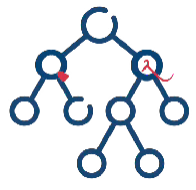
\includegraphics[height=0.9cm]{msca_logo.png}}%
  \end{center}
  \vspace{0.45cm}
  \begin{center}
    \begin{minipage}{0.1\textwidth}\centering
      \href{https://quantlet.com}{
\includegraphics[height=0.9cm]{ql_logo.png}}\end{minipage}%
    \begin{minipage}{0.78\textwidth}\centering
      {\Large\bfseries\usebeamercolor[fg]{title}\inserttitle}\par\vspace{0.25cm}
      {\large\usebeamercolor[fg]{title}\insertsubtitle}\end{minipage}%
    \begin{minipage}{0.1\textwidth}\centering
      \href{https://quantinar.com}{
\includegraphics[height=0.9cm]{qr_logo.png}}\end{minipage}
  \end{center}
  \vfill
  \hspace{0.4cm}{\bfseries\insertauthor}\par\vspace{0.12cm}
  \hspace{0.4cm}\begin{minipage}[t]{0.92\textwidth}\raggedright\footnotesize\insertinstitute\end{minipage}
  \par\vspace{0.4cm}}

% ---------------------------------------------------------------- lecture metadata
\newcommand{\nnshort}{}
\newcommand{\nnnb}{notebooks}
\newcommand{\nnrepo}{https://github.com/danpele/NEURAL_BIZ/tree/main}
% language-dependent labels (English default; \nnromanian switches to Romanian, call it before \nnlecture)
\newcommand{\txtcourse}{Neural Networks and Deep Learning}
\newcommand{\txtlecture}{Lecture}
\newcommand{\txtoutline}{Outline}
\newcommand{\txtintuition}{In one sentence:}
\newcommand{\txtjob}{In practice:}
\newcommand{\txttry}{Experiment yourself:}
\newcommand{\txtwhere}{where}
\newcommand{\txtsim}{SIMULATED DATA (teaching illustration)}
\newcommand{\txtnbsuffix}{}
\newcommand{\txtinstitute}{Bucharest University of Economic Studies (ASE), Department of Statistics and Econometrics\\
    Romanian Academy, Institute for Economic Forecasting (IPE)\\
    IDA Institute Digital Assets \textbullet\ AI4EFin \textbullet\ MSCA Digital Finance}
\newcommand{\nnromanian}{%
  \renewcommand{\txtcourse}{Rețele neuronale și deep learning}%
  \renewcommand{\txtlecture}{Cursul}%
  \renewcommand{\txtoutline}{Cuprins}%
  \renewcommand{\txtintuition}{Pe scurt:}%
  \renewcommand{\txtjob}{În practică:}%
  \renewcommand{\txttry}{Exercițiu practic:}%
  \renewcommand{\txtwhere}{unde}%
  \renewcommand{\txtsim}{DATE SIMULATE (doar pentru ilustrare)}%
  \renewcommand{\txtnbsuffix}{\string_ro}%
  \renewcommand{\txtinstitute}{Academia de Studii Economice din București (ASE), Departamentul de Statistică și Econometrie\\
    Academia Română, Institutul de Prognoză Economică (IPE)\\
    IDA Institute Digital Assets \textbullet\ AI4EFin \textbullet\ MSCA Digital Finance}}
\newcommand{\nnlecture}[2]{%
  \renewcommand{\nnshort}{\txtlecture\ #1}%
  \renewcommand{\nnnb}{notebooks/L#1\string_notebook\txtnbsuffix.ipynb}%
  \title[NN]{\txtcourse}%
  \subtitle{\txtlecture\ #1: #2}%
  \author{Prof.\ dr.\ Daniel Traian PELE}%
  \institute{\txtinstitute}%
  \date{}}

% ---------------------------------------------------------------- teaching blocks (one message per frame)
% \intuition{one plain sentence}  ->  formula with every symbol defined  ->  real-data example  ->  \manager{one line}
\newcommand{\intuition}[1]{\begin{itemize}\item {\color{MainBlue}\textbf{\txtintuition}}~#1\end{itemize}\vspace{0.6mm}}
\newcommand{\manager}[1]{\colorbox{Forest!10}{\parbox{\dimexpr\linewidth-2\fboxsep\relax}{\footnotesize
  \begin{itemize}\setlength{\itemsep}{0pt}\item \textbf{\color{Forest}\txtjob}~#1\end{itemize}}}}
% Experiment yourself: pointer to the matching notebook section
\newcommand{\tryit}[1]{{\scriptsize\href{\nnrepo/\nnnb}{%
  \raisebox{-0.15em}{
\includegraphics[height=0.85em]{ql_logo.png}}\,\textbf{\txttry}~\color{MainBlue}#1}}}
% bottom row: manager line (left) + experiment pointer (right), pinned to the bottom of the frame
\newcommand{\bottomrow}[2]{\par\vfill\noindent\begin{minipage}[b]{0.72\linewidth}#1\end{minipage}\hfill
  \begin{minipage}[b]{0.26\linewidth}\raggedleft #2\end{minipage}\par\vspace{0.5mm}}
\newcommand{\where}[1]{{\footnotesize\textbf{\txtwhere}~#1\par}}

% ---------------------------------------------------------------- helpers
% chart source line under a figure: \chartsource{Source ...; period ...}
\newcommand{\chartsource}[1]{\par\vspace{1pt}{\scriptsize\color{FooterGray}#1\par}}
% link to code: \quantlet{label}{path inside the repo}
\newcommand{\quantlet}[2]{\par\vspace{1pt}\hfill\href{\nnrepo/#2}{%
  \raisebox{-0.15em}{
\includegraphics[height=0.75em]{ql_logo.png}}\textcolor{MainBlue}{\scriptsize\ #1}}}
% inline Quantlet link for the bottom-right corner of a frame: \qlink{label}{path inside the repo}
\newcommand{\qlink}[2]{{\scriptsize\href{\nnrepo/#2}{\raisebox{-0.15em}{
\includegraphics[height=0.85em]{ql_logo.png}}\,\textcolor{MainBlue}{#1}}}}
\newcommand{\simlabel}{\colorbox{Crimson!12}{\scriptsize\bfseries\color{Crimson}\txtsim}}
\newcommand{\E}{\mathbb{E}}
\newcommand{\Var}{\operatorname{Var}}
\newcommand{\Cov}{\operatorname{Cov}}
\newcommand{\Corr}{\operatorname{Corr}}
\newcommand{\asinh}{\operatorname{asinh}}
\newcommand{\iid}{\overset{\text{i.i.d.}}{\sim}}
\newcommand{\EUR}{EUR}
% deep-learning notation (Bishop & Bishop, 2024): vectors bold lower case, matrices bold upper case
\newcommand{\R}{\mathbb{R}}
\newcommand{\vx}{\mathbf{x}}
\newcommand{\vy}{\mathbf{y}}
\newcommand{\vz}{\mathbf{z}}
\newcommand{\vh}{\mathbf{h}}
\newcommand{\vw}{\mathbf{w}}
\newcommand{\vb}{\mathbf{b}}
\newcommand{\mW}{\mathbf{W}}
\newcommand{\mX}{\mathbf{X}}
\newcommand{\btheta}{\boldsymbol{\theta}}
\newcommand{\loss}{\mathcal{L}}
\newcommand{\dataset}{\mathcal{D}}
\DeclareMathOperator*{\argmin}{arg\,min}
\DeclareMathOperator*{\argmax}{arg\,max}
\DeclareMathOperator{\softmax}{softmax}
\DeclareMathOperator{\ReLU}{ReLU}
\DeclareMathOperator{\sigm}{\sigma}

%   \nnlecture{k}{Lecture title}
% Logos live in lectures/common/logos/, charts in lectures/Lk/charts/.
% Do NOT add \hfuzz / \vfuzz / \hbadness here: overfull boxes must be fixed, not hidden.
% =============================================================================

\usetheme{default}
\setbeamersize{text margin left=7mm, text margin right=7mm}

% ---------------------------------------------------------------- packages
\usepackage[utf8]{inputenc}
\usepackage[T1]{fontenc}
\usepackage{lmodern}
\usepackage{amsmath, amssymb}
\usepackage{mathtools}
\usepackage{bm}
\usepackage{tikz}
\usetikzlibrary{arrows.meta, positioning, calc, shapes.misc}
\usepackage{booktabs}
\usepackage{array}
\usepackage{graphicx}
\usepackage{colortbl}
\usepackage{xcolor}
\usepackage{multicol}
\hypersetup{colorlinks=true, linkcolor=MainBlue, urlcolor=MainBlue, citecolor=MainBlue}
\graphicspath{{../common/logos/}}   % charts are included with their language folder: charts/en/, charts/ro/

% ---------------------------------------------------------------- colours
\definecolor{MainBlue}{RGB}{26, 58, 110}
\definecolor{IDAred}{RGB}{205, 0, 0}
\definecolor{DarkGray}{RGB}{51, 51, 51}
\definecolor{FooterGray}{RGB}{100, 100, 100}
\definecolor{BlockGray}{RGB}{236, 238, 242}
\definecolor{KeynoteGray}{RGB}{218, 218, 218}
\definecolor{Crimson}{RGB}{190, 40, 50}
\definecolor{Forest}{RGB}{30, 110, 50}
\definecolor{Bitter}{RGB}{214, 150, 20}
% chart palette (same hex values and order as lectures/common/nn_plot.py SERIES)
\definecolor{Ser1}{HTML}{2A78D6}
\definecolor{Ser2}{HTML}{EB6834}
\definecolor{Ser3}{HTML}{1BAF7A}
\definecolor{Ser4}{HTML}{EDA100}
\definecolor{Ser5}{HTML}{E87BA4}
\definecolor{Ser6}{HTML}{008300}
\definecolor{Ser7}{HTML}{6250D6}
\definecolor{Ser8}{HTML}{E34948}

\setbeamertemplate{background}{%
  \begin{tikzpicture}[remember picture, overlay]
    \shade[shading=axis, shading angle=315, top color=white, bottom color=KeynoteGray]
      (current page.south west) rectangle (current page.north east);
  \end{tikzpicture}}
\setbeamercolor{background canvas}{bg=}
\setbeamercolor{structure}{fg=MainBlue}
\setbeamercolor{normal text}{fg=DarkGray}
\setbeamercolor{title}{fg=IDAred}
\setbeamercolor{frametitle}{fg=IDAred, bg=}
\setbeamercolor{block title}{bg=MainBlue, fg=white}
\setbeamercolor{block body}{bg=BlockGray, fg=DarkGray}
\setbeamercolor{block title alerted}{bg=Crimson, fg=white}
\setbeamercolor{block body alerted}{bg=Crimson!7, fg=DarkGray}
\setbeamercolor{block title example}{bg=Forest, fg=white}
\setbeamercolor{block body example}{bg=Forest!7, fg=DarkGray}
\setbeamercolor{item}{fg=MainBlue}
\setbeamerfont{frametitle}{size=\large, series=\bfseries}
\setbeamerfont{block title}{size=\small, series=\bfseries}
\setbeamertemplate{blocks}[rounded][shadow=false]
\setbeamertemplate{itemize item}{\color{MainBlue}$\boxdot$}
\setbeamertemplate{itemize subitem}{\color{MainBlue}\scriptsize$\blacktriangleright$}
% compact two-level lists: level 1 = main point, level 2 = details (no text outside bullets)
\setbeamerfont{itemize/enumerate subbody}{size=\footnotesize}
\setlength{\leftmargini}{1.1em}
\setlength{\leftmarginii}{1.1em}
\setbeamertemplate{itemize/enumerate body begin}{\setlength{\topsep}{0pt}\setlength{\partopsep}{0pt}\setlength{\parskip}{0pt}}
\setbeamertemplate{itemize/enumerate subbody begin}{\setlength{\topsep}{0pt}\setlength{\partopsep}{0pt}\setlength{\itemsep}{0pt}\vspace{-0.4ex}}

\setbeamertemplate{enumerate item}{\color{MainBlue}\insertenumlabel.}
\setlength{\leftmargini}{1.3em}
\setlength{\leftmarginii}{1.2em}
\setbeamertemplate{navigation symbols}{}
\setbeamertemplate{section in toc}{\color{MainBlue}$\blacktriangleright$~\inserttocsection}
\setbeamertemplate{caption}{\raggedright\insertcaption\par}
% frame subtitle = precise citation line under the claim title (Weron style)
\setbeamerfont{framesubtitle}{size=\footnotesize}
\setbeamercolor{framesubtitle}{fg=FooterGray}
% outline that reappears at every section with the current section highlighted
\setbeamertemplate{section in toc shaded}[default][35]
\setbeamertemplate{subsection in toc shaded}[default][35]
\setbeamertemplate{subsection in toc}{\leavevmode\leftskip=2.2em\color{DarkGray}\small\inserttocsubsection\par}
\AtBeginSection[]{{\begin{frame}{\txtoutline}\vspace{2mm}\small
  \tableofcontents[currentsection,hideothersubsections]\end{frame}}}

% ---------------------------------------------------------------- head and foot
\setbeamertemplate{headline}{%
  \vskip10pt%
  \hbox to \paperwidth{\hskip0.5cm%
    {\small\color{FooterGray}\renewcommand{\hyperlink}[2]{##2}\insertsectionhead}%
    \hfill\textcolor{FooterGray}{\small\insertframenumber}\hskip0.5cm}%
  \vskip4pt{\color{FooterGray}\hrule height 0.4pt}}
% footer as in the other courses (MFM, SFM): course name on the left, small sparkline on the right
\setbeamertemplate{footline}{%
  {\color{FooterGray}\hrule height 0.4pt}\vskip4pt%
  \hbox to \paperwidth{\hskip0.5cm%
    \textcolor{FooterGray}{\small\txtcourse}%
    \hfill\raisebox{-0.1em}{\begin{tikzpicture}[x=0.08em, y=0.08em, line width=0.4pt]
      \draw[FooterGray] (0,3) -- (1,4) -- (2,3.5) -- (3,5) -- (4,4) -- (5,6) -- (6,5.5) -- (7,4) -- (8,5) -- (9,7) -- (10,6) -- (11,5) -- (12,6.5) -- (13,8) -- (14,7) -- (15,6) -- (16,7.5) -- (17,9) -- (18,8) -- (19,7) -- (20,8.5) -- (21,10) -- (22,9) -- (23,8) -- (24,9.5);
    \end{tikzpicture}}\hskip0.5cm}%
  \vskip6pt}

% ---------------------------------------------------------------- title page
\defbeamertemplate*{title page}{nn}[1][]{%
  \vspace{0.15cm}
  \begin{center}
    \href{https://www.ase.ro}{
\includegraphics[height=0.9cm]{ase_logo.png}}\hspace{0.3cm}%
    \href{https://ipe.ro/new}{
\includegraphics[height=0.9cm]{acad_logo.png}}\hspace{0.3cm}%
    \href{https://theida.net}{
\includegraphics[height=0.9cm]{ida_logo.png}}\hspace{0.3cm}%
    \href{https://blockchain-research-center.com}{
\includegraphics[height=0.9cm]{brc_logo.png}}\hspace{0.3cm}%
    \href{https://www.ai4efin.ase.ro}{
\includegraphics[height=0.9cm]{ai4efin_logo.png}}\hspace{0.3cm}%
    \href{https://www.digital-finance-msca.com}{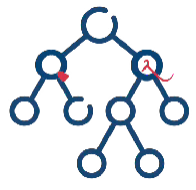
\includegraphics[height=0.9cm]{msca_logo.png}}%
  \end{center}
  \vspace{0.45cm}
  \begin{center}
    \begin{minipage}{0.1\textwidth}\centering
      \href{https://quantlet.com}{
\includegraphics[height=0.9cm]{ql_logo.png}}\end{minipage}%
    \begin{minipage}{0.78\textwidth}\centering
      {\Large\bfseries\usebeamercolor[fg]{title}\inserttitle}\par\vspace{0.25cm}
      {\large\usebeamercolor[fg]{title}\insertsubtitle}\end{minipage}%
    \begin{minipage}{0.1\textwidth}\centering
      \href{https://quantinar.com}{
\includegraphics[height=0.9cm]{qr_logo.png}}\end{minipage}
  \end{center}
  \vfill
  \hspace{0.4cm}{\bfseries\insertauthor}\par\vspace{0.12cm}
  \hspace{0.4cm}\begin{minipage}[t]{0.92\textwidth}\raggedright\footnotesize\insertinstitute\end{minipage}
  \par\vspace{0.4cm}}

% ---------------------------------------------------------------- lecture metadata
\newcommand{\nnshort}{}
\newcommand{\nnnb}{notebooks}
\newcommand{\nnrepo}{https://github.com/danpele/NEURAL_BIZ/tree/main}
% language-dependent labels (English default; \nnromanian switches to Romanian, call it before \nnlecture)
\newcommand{\txtcourse}{Neural Networks and Deep Learning}
\newcommand{\txtlecture}{Lecture}
\newcommand{\txtoutline}{Outline}
\newcommand{\txtintuition}{In one sentence:}
\newcommand{\txtjob}{In practice:}
\newcommand{\txttry}{Experiment yourself:}
\newcommand{\txtwhere}{where}
\newcommand{\txtsim}{SIMULATED DATA (teaching illustration)}
\newcommand{\txtnbsuffix}{}
\newcommand{\txtinstitute}{Bucharest University of Economic Studies (ASE), Department of Statistics and Econometrics\\
    Romanian Academy, Institute for Economic Forecasting (IPE)\\
    IDA Institute Digital Assets \textbullet\ AI4EFin \textbullet\ MSCA Digital Finance}
\newcommand{\nnromanian}{%
  \renewcommand{\txtcourse}{Rețele neuronale și deep learning}%
  \renewcommand{\txtlecture}{Cursul}%
  \renewcommand{\txtoutline}{Cuprins}%
  \renewcommand{\txtintuition}{Pe scurt:}%
  \renewcommand{\txtjob}{În practică:}%
  \renewcommand{\txttry}{Exercițiu practic:}%
  \renewcommand{\txtwhere}{unde}%
  \renewcommand{\txtsim}{DATE SIMULATE (doar pentru ilustrare)}%
  \renewcommand{\txtnbsuffix}{\string_ro}%
  \renewcommand{\txtinstitute}{Academia de Studii Economice din București (ASE), Departamentul de Statistică și Econometrie\\
    Academia Română, Institutul de Prognoză Economică (IPE)\\
    IDA Institute Digital Assets \textbullet\ AI4EFin \textbullet\ MSCA Digital Finance}}
\newcommand{\nnlecture}[2]{%
  \renewcommand{\nnshort}{\txtlecture\ #1}%
  \renewcommand{\nnnb}{notebooks/L#1\string_notebook\txtnbsuffix.ipynb}%
  \title[NN]{\txtcourse}%
  \subtitle{\txtlecture\ #1: #2}%
  \author{Prof.\ dr.\ Daniel Traian PELE}%
  \institute{\txtinstitute}%
  \date{}}

% ---------------------------------------------------------------- teaching blocks (one message per frame)
% \intuition{one plain sentence}  ->  formula with every symbol defined  ->  real-data example  ->  \manager{one line}
\newcommand{\intuition}[1]{\begin{itemize}\item {\color{MainBlue}\textbf{\txtintuition}}~#1\end{itemize}\vspace{0.6mm}}
\newcommand{\manager}[1]{\colorbox{Forest!10}{\parbox{\dimexpr\linewidth-2\fboxsep\relax}{\footnotesize
  \begin{itemize}\setlength{\itemsep}{0pt}\item \textbf{\color{Forest}\txtjob}~#1\end{itemize}}}}
% Experiment yourself: pointer to the matching notebook section
\newcommand{\tryit}[1]{{\scriptsize\href{\nnrepo/\nnnb}{%
  \raisebox{-0.15em}{
\includegraphics[height=0.85em]{ql_logo.png}}\,\textbf{\txttry}~\color{MainBlue}#1}}}
% bottom row: manager line (left) + experiment pointer (right), pinned to the bottom of the frame
\newcommand{\bottomrow}[2]{\par\vfill\noindent\begin{minipage}[b]{0.72\linewidth}#1\end{minipage}\hfill
  \begin{minipage}[b]{0.26\linewidth}\raggedleft #2\end{minipage}\par\vspace{0.5mm}}
\newcommand{\where}[1]{{\footnotesize\textbf{\txtwhere}~#1\par}}

% ---------------------------------------------------------------- helpers
% chart source line under a figure: \chartsource{Source ...; period ...}
\newcommand{\chartsource}[1]{\par\vspace{1pt}{\scriptsize\color{FooterGray}#1\par}}
% link to code: \quantlet{label}{path inside the repo}
\newcommand{\quantlet}[2]{\par\vspace{1pt}\hfill\href{\nnrepo/#2}{%
  \raisebox{-0.15em}{
\includegraphics[height=0.75em]{ql_logo.png}}\textcolor{MainBlue}{\scriptsize\ #1}}}
% inline Quantlet link for the bottom-right corner of a frame: \qlink{label}{path inside the repo}
\newcommand{\qlink}[2]{{\scriptsize\href{\nnrepo/#2}{\raisebox{-0.15em}{
\includegraphics[height=0.85em]{ql_logo.png}}\,\textcolor{MainBlue}{#1}}}}
\newcommand{\simlabel}{\colorbox{Crimson!12}{\scriptsize\bfseries\color{Crimson}\txtsim}}
\newcommand{\E}{\mathbb{E}}
\newcommand{\Var}{\operatorname{Var}}
\newcommand{\Cov}{\operatorname{Cov}}
\newcommand{\Corr}{\operatorname{Corr}}
\newcommand{\asinh}{\operatorname{asinh}}
\newcommand{\iid}{\overset{\text{i.i.d.}}{\sim}}
\newcommand{\EUR}{EUR}
% deep-learning notation (Bishop & Bishop, 2024): vectors bold lower case, matrices bold upper case
\newcommand{\R}{\mathbb{R}}
\newcommand{\vx}{\mathbf{x}}
\newcommand{\vy}{\mathbf{y}}
\newcommand{\vz}{\mathbf{z}}
\newcommand{\vh}{\mathbf{h}}
\newcommand{\vw}{\mathbf{w}}
\newcommand{\vb}{\mathbf{b}}
\newcommand{\mW}{\mathbf{W}}
\newcommand{\mX}{\mathbf{X}}
\newcommand{\btheta}{\boldsymbol{\theta}}
\newcommand{\loss}{\mathcal{L}}
\newcommand{\dataset}{\mathcal{D}}
\DeclareMathOperator*{\argmin}{arg\,min}
\DeclareMathOperator*{\argmax}{arg\,max}
\DeclareMathOperator{\softmax}{softmax}
\DeclareMathOperator{\ReLU}{ReLU}
\DeclareMathOperator{\sigm}{\sigma}

\usepackage[romanian]{babel}
\nnromanian
\nnlecture{8}{Modele generative: autoencodere, VAE, GAN, difuzie}
\begin{document}
{\setbeamertemplate{headline}{}\setbeamertemplate{footline}{}
\begin{frame}\titlepage\end{frame}}
% END-FRONT-MATTER

\begin{frame}{Obiectivele cursului}
\small
\begin{itemize}\setlength{\itemsep}{5pt}
  \item Diferența dintre un model discriminativ $p(y\mid\mathbf x)$ și un model generativ $p(\mathbf x)$
    \begin{itemize}\setlength{\itemsep}{0pt}
      \item De ce finanțele au nevoie de amîndouă
    \end{itemize}
  \item Derivarea și antrenarea a patru familii de modele
    \begin{itemize}\setlength{\itemsep}{0pt}
      \item Autoencoderul (AE), autoencoderul variațional (VAE), rețeaua generativă adversarială (GAN) și modelul probabilistic de difuzie (DDPM)
    \end{itemize}
  \item Aplicarea lor pe date reale
    \begin{itemize}\setlength{\itemsep}{0pt}
      \item Detectarea fraudei cu carduri, imagini de îmbrăcăminte în formatul cifrelor Modified National Institute of Standards and Technology (MNIST), randamentele S\&P 500 și curba randamentelor din zona euro, fiecare comparat cu un model clasic
    \end{itemize}
  \item Evaluarea datelor sintetice
    \begin{itemize}\setlength{\itemsep}{0pt}
      \item Cozile distribuției, gruparea volatilității, măsuri de risc precum valoarea la risc (VaR) și ce nu poate reproduce un generator
    \end{itemize}
\end{itemize}
\end{frame}

% BEGIN-ABBR

\begin{frame}{Abrevieri}
\small
\vspace{-1mm}\begin{columns}[T,onlytextwidth]
\begin{column}{0.49\textwidth}{\scriptsize\renewcommand{\arraystretch}{0.96}\begin{tabular}{@{}>{\bfseries}l@{\ \ }p{0.74\linewidth}@{}}AE & autoencoder (rețea de autocodificare)\\
ASE & Academia de Studii Economice din București\\
DDPM & model probabilistic de difuzie cu eliminarea zgomotului (denoising diffusion)\\
ELBO & marginea inferioară a verosimilității (evidence lower bound)\\
ES & pierderea așteptată în coadă (expected shortfall)\\
GAN & rețea generativă adversarială\\
IPE & Institutul de Prognoză Economică, Academia Română\\
JS & divergența Jensen--Shannon\\
KL & divergența Kullback--Leibler\\
LLM & model mare de limbaj\\
MLP & perceptron multistrat\\\end{tabular}}\end{column}
\begin{column}{0.49\textwidth}{\scriptsize\renewcommand{\arraystretch}{0.96}\begin{tabular}{@{}>{\bfseries}l@{\ \ }p{0.74\linewidth}@{}}MNIST & cifrele scrise de mînă ale Modified National Institute of Standards and Technology\\
PCA & analiza componentelor principale\\
PR-AUC & aria de sub curba precizie-recall\\
ReLU & unitate liniară rectificată (rectified linear unit)\\
ROC & caracteristica de operare a receptorului (receiver operating characteristic)\\
ROC-AUC & aria de sub curba ROC\\
TSTR & antrenare pe date sintetice, test pe date reale (train on synthetic, test on real)\\
VAE & autoencoder variațional\\
VaR & valoarea la risc (Value-at-Risk)\\
WGAN & GAN Wasserstein\\\end{tabular}}\end{column}
\end{columns}
\end{frame}

% END-ABBR


\section{Principiile modelării generative}

\begin{frame}{Un model generativ învață cum apar datele}
\footnotesize
\intuition{Un clasificator învață granița dintre clase; un model generativ învață toată distribuția datelor.}
\begin{columns}[T,onlytextwidth]
\begin{column}{0.58\textwidth}
\[ \underbrace{p(y\mid\mathbf x)}_{\text{discriminativ}}\qquad\text{vs.}\qquad\underbrace{p(\mathbf x)\ \text{sau}\ p(\mathbf x,y)=p(\mathbf x\mid y)\,p(y)}_{\text{generativ}} \]\[ \hat\btheta=\argmax_{\btheta}\ \sum_{i=1}^{n}\log p_{\btheta}(\mathbf x_i) \]{\footnotesize\begin{itemize}\setlength{\itemsep}{0pt}
  \item \textbf{\txtwhere}
    \begin{itemize}\setlength{\itemsep}{0pt}
      \item $\mathbf x$ = o observație (tranzacție, imagine, zi de randamente, curbă)
      \item $y$ = o etichetă
      \item $p_{\btheta}$ = densitatea modelului, estimată prin verosimilitate maximă.
    \end{itemize}
\end{itemize}\par}
\end{column}
\begin{column}{0.39\textwidth}
\begin{itemize}\setlength{\itemsep}{3pt}
  \item \textbf{Patru utilizări în finanțe}
    \begin{itemize}\setlength{\itemsep}{0pt}
      \item Detectarea anomaliilor: $p(\mathbf x)$ mic = suspect (fraudă)
      \item Scenarii pentru teste de stres și măsuri de risc
      \item Date sintetice partajate fără înregistrări despre clienți
    \end{itemize}
\end{itemize}
\end{column}
\end{columns}
\par\vfill\manager{un clasificator ordonează clienții, un model generativ arată și ce s-ar putea întîmpla.}\par\vspace{0.5mm}
\par\vfill\noindent{\scriptsize\color{FooterGray}(Bishop \& Bishop, 2024, ch.\ 16)}\par\vspace{0.5mm}
\end{frame}

\begin{frame}{Modele cu variabile latente}
\footnotesize
\intuition{Unsprezece randamente sau 784 de pixeli sînt determinate de cîțiva factori ascunși; un model cu variabile latente formalizează acest lucru.}
\begin{columns}[T,onlytextwidth]
\begin{column}{0.58\textwidth}
\[ p_{\btheta}(\mathbf x)=\int p_{\btheta}(\mathbf x\mid\mathbf z)\,p(\mathbf z)\,d\mathbf z,\qquad \mathbf z\in\R^k,\ k\ll d \]\[ \text{liniar-gaussian:}\ \ \mathbf x=W\mathbf z+\boldsymbol\mu+\boldsymbol\varepsilon,\ \mathbf z\sim\mathcal N(0,I),\ \boldsymbol\varepsilon\sim\mathcal N(0,\sigma^2I) \]{\footnotesize\begin{itemize}\setlength{\itemsep}{0pt}
  \item \textbf{\txtwhere}
    \begin{itemize}\setlength{\itemsep}{0pt}
      \item $\mathbf z$ = factorii latenți, în număr de $k$
      \item $d$ = dimensiunea datelor
      \item Cazul liniar-gaussian este analiza probabilistă a componentelor principale (PCA), cu verosimilitate în formă închisă
      \item Cu un decodor neuronal integrala nu mai are formă închisă.
    \end{itemize}
\end{itemize}\par}
\end{column}
\begin{column}{0.39\textwidth}
\begin{itemize}\setlength{\itemsep}{3pt}
  \item \textbf{Curba randamentelor}
    \begin{itemize}\setlength{\itemsep}{0pt}
      \item Nivel, pantă, curbură: trei factori explică majoritatea mișcărilor zilnice
    \end{itemize}
  \item \textbf{Prețul neliniarității}
    \begin{itemize}\setlength{\itemsep}{0pt}
      \item VAE: o margine inferioară pentru $\log p$; GAN: nicio verosimilitate; difuzia: o margine construită pas cu pas
    \end{itemize}
\end{itemize}
\end{column}
\end{columns}
\par\vfill\manager{la evaluarea unui model, întrebați care parte este povestea latentă și care este zgomot estimat.}\par\vspace{0.5mm}
\par\vfill\noindent{\scriptsize\color{FooterGray}(Bishop \& Bishop, 2024, sec.\ 16.2)}\par\vspace{0.5mm}
\end{frame}

\begin{frame}{Patru familii de modele generative}
\footnotesize
{\scriptsize\renewcommand{\arraystretch}{1.25}\setlength{\tabcolsep}{4pt}
\begin{tabular}{@{}p{0.15\textwidth}p{0.20\textwidth}p{0.17\textwidth}p{0.17\textwidth}p{0.23\textwidth}@{}}\toprule
Familia & Ce se optimizează & Verosimilitate & Generarea & În acest curs \\ \midrule
AE & eroarea de reconstrucție & nu & nu este generator & frauda cu carduri ca anomalie \\
VAE & marginea inferioară a verosimilității & margine inferioară & o trecere, imagini neclare & imagini de îmbrăcăminte; curbe ale randamentelor \\
GAN & joc contra unui discriminator & nu & o trecere, imagini clare & randamentele zilnice S\&P 500 \\
DDPM & eroarea de eliminare a zgomotului & margine inferioară & mulți pași, fidel & curbele randamentelor din zona euro \\
\bottomrule\end{tabular}}
\vspace{2mm}
\begin{itemize}\setlength{\itemsep}{2pt}
  \item \textbf{Nimic nu este gratuit}: verosimilitatea, calitatea eșantioanelor și viteza rareori vin împreună
    \begin{itemize}\setlength{\itemsep}{0pt}
      \item Alegerea depinde de utilizare
    \end{itemize}
  \item \textbf{Fluxurile de normalizare} (verosimilitate exactă, rețele inversabile) completează tabloul
    \begin{itemize}\setlength{\itemsep}{0pt}
      \item Vezi Bishop \& Bishop (2024), cap.\ 18
    \end{itemize}
\end{itemize}
\par\vfill\noindent{\scriptsize\color{FooterGray}(Bishop \& Bishop, 2024, ch.\ 17--20)}\par\vspace{0.5mm}
\end{frame}


\section{Autoencodere: detectarea anomaliilor la fraude cu carduri}

\begin{frame}{Un autoencoder comprimă datele printr-un strat îngust și le reconstruiește}
\footnotesize
\intuition{Dacă rețeaua reconstruiește tranzacțiile normale din cîteva numere, una pe care nu o poate reconstrui este neobișnuită.}
\begin{columns}[T,onlytextwidth]
\begin{column}{0.58\textwidth}
\[ \mathbf z=f_{\phi}(\mathbf x)\in\R^{k},\qquad \hat{\mathbf x}=g_{\psi}(\mathbf z) \]\[ \min_{\phi,\psi}\ \frac1n\sum_{i=1}^{n}\big\|\mathbf x_i-g_{\psi}(f_{\phi}(\mathbf x_i))\big\|^2,\qquad s(\mathbf x)=\tfrac1d\|\mathbf x-\hat{\mathbf x}\|^2 \]{\footnotesize\begin{itemize}\setlength{\itemsep}{0pt}
  \item \textbf{\txtwhere}
    \begin{itemize}\setlength{\itemsep}{0pt}
      \item $f_\phi$, $g_\psi$ = codificatorul și decodorul, perceptroni multistrat mici (MLP) cu unități liniare rectificate (ReLU)
      \item $k$ = dimensiunea stratului îngust
      \item $s(\mathbf x)$ = scorul de anomalie
      \item Cu $f,g$ liniare se obține subspațiul PCA.
    \end{itemize}
\end{itemize}\par}
\end{column}
\begin{column}{0.39\textwidth}
\begin{itemize}\setlength{\itemsep}{3pt}
  \item \textbf{Autoencoderul nostru}
    \begin{itemize}\setlength{\itemsep}{0pt}
      \item 29 de intrări (28 de componente anonimizate + logaritmul sumei) $\to$ 16 $\to$ 8 $\to$ 16 $\to$ 29
      \item 1\,253 de parametri, antrenat numai pe tranzacții legitime
    \end{itemize}
  \item \textbf{Nu are nevoie de etichete}: util pentru fraude noi sau neconfirmate
\end{itemize}
\end{column}
\end{columns}
\par\vfill\manager{un autoencoder modelează ``normalul'' și semnalează ce diferă, nu neapărat ce este infracțional.}\par\vspace{0.5mm}
\par\vfill\noindent{\scriptsize\color{FooterGray}(Bishop \& Bishop, 2024, ch.\ 19)}\hfill\tryit{notebook, secțiunea 1}\par\vspace{0.5mm}
\end{frame}

\begin{frame}{Experimentul de fraudă: două zile de plăți cu cardul, împărțite în timp}
\footnotesize
{\scriptsize\renewcommand{\arraystretch}{1.05}\setlength{\tabcolsep}{4pt}
\begin{tabular}{@{}p{0.27\textwidth}p{0.66\textwidth}@{}}\toprule
Element & Alegerea \\ \midrule
Date & tranzacțiile cu carduri ULB (Dal Pozzolo et al., 2015): 28\,924 de rînduri = toate cele 492 de fraude și 10\,\% dintre cele legitime, reponderate la datele complete \\
Împărțire în timp & primele 60\,\% din interval = antrenare (numai legitime, 16\,994 de rînduri), următoarele 20\,\% = validare, ultimele 20\,\% = test \\
Test & 57\,174 de tranzacții din datele complete, 75 de fraude (0{,}131\,\%) \\
Modele de referință & PCA cu 8 componente (autoencoder liniar); regresie logistică antrenată \textit{cu} etichetele de fraudă \\
Măsuri & aria de sub curba precizie-recall (PR-AUC) și aria de sub curba caracteristicii de operare a receptorului (ROC-AUC), ponderate la datele complete; fraudele printre primele 0,1\,\% scoruri \\
\bottomrule\end{tabular}}
\vspace{1mm}
\begin{itemize}\setlength{\itemsep}{2pt}
  \item \textbf{Fără scurgeri de informație}: mediile și abaterile standard din tranzacțiile legitime de antrenare
    \begin{itemize}\setlength{\itemsep}{0pt}
      \item Oprire timpurie pe partea de validare
      \item Semințele 1--3
    \end{itemize}
\end{itemize}
\par\vfill\noindent{\scriptsize\color{FooterGray}(Dal Pozzolo et al., 2015)}\hfill\tryit{notebook, secțiunea 1}\par\vspace{0.5mm}
\end{frame}

\begin{frame}{Eroarea de reconstrucție a plăților frauduloase și a celor legitime}
\small
\begin{center}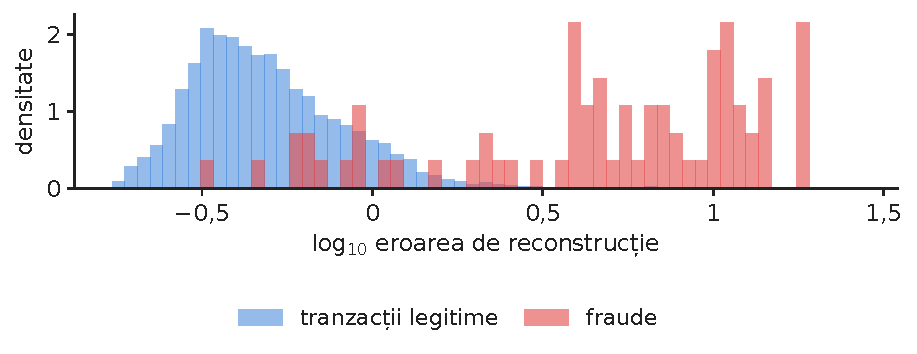
\includegraphics[width=\textwidth,height=0.510\textheight,keepaspectratio]{charts/ro/ae_error_dist.pdf}\end{center}\vspace{-3mm}
\chartsource{Sursa: ULB Machine Learning Group și Worldline, tranzacții cu carduri (OpenML 1597). Date: estimări proprii; două zile din septembrie 2013; test = ultimele 20\,\% din interval.}
\vspace{0.5mm}
\begin{itemize}\setlength{\itemsep}{0pt}
  \item \textbf{Separarea}: eroarea mediană a unei fraude este de 12{,}7 ori mai mare decît a unei tranzacții legitime (partea de test)
  \item \textbf{Suprapunerea}: multe fraude arată totuși normal pentru autoencoder
    \begin{itemize}\setlength{\itemsep}{0pt}
      \item Se află în grosul distribuției legitime
    \end{itemize}
\end{itemize}
\par\vfill\noindent{\scriptsize\color{FooterGray}}\hfill\qlink{NN\_L8\_ae\_error\_dist}{Quantlets/L8/NN_L8_ae_error_dist}\par\vspace{0.5mm}
\end{frame}

\begin{frame}{Autoencoderul fără etichete comparat cu un clasificator supervizat}
\small
\begin{center}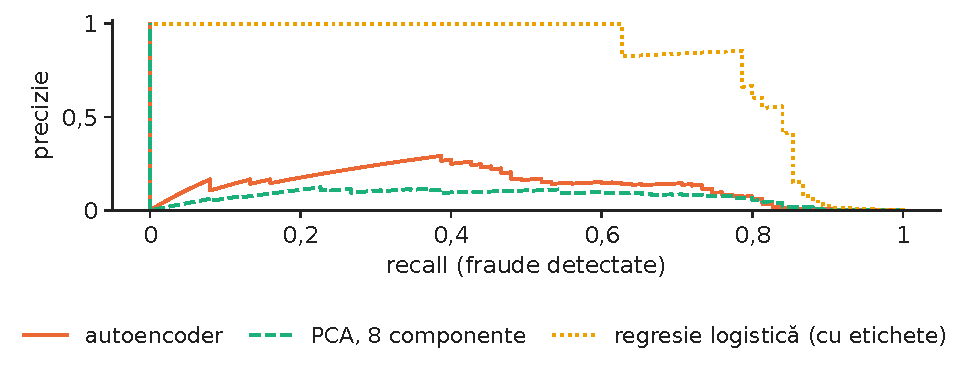
\includegraphics[width=\textwidth,height=0.461\textheight,keepaspectratio]{charts/ro/ae_pr.pdf}\end{center}\vspace{-3mm}
\chartsource{Sursa: ULB Machine Learning Group și Worldline, tranzacții cu carduri (OpenML 1597). Date: estimări proprii; două zile din septembrie 2013; test = ultimele 20\,\% din interval.}
\vspace{0.5mm}
\begin{itemize}\setlength{\itemsep}{0pt}
  \item \textbf{PR-AUC pe partea de test}: autoencoder 14{,}2\,\% (abatere standard 2{,}9 pe 3 semințe), PCA 7{,}6\,\%, regresie logistică cu etichete 80{,}4\,\%
    \begin{itemize}\setlength{\itemsep}{0pt}
      \item Un scor aleator: 0{,}131\,\%
    \end{itemize}
  \item \textbf{ROC-AUC} este mare pentru toate trei (94{,}4, 95{,}3, 98{,}2\,\%): la o fraudă din 700 ascunde diferența pe care o arată PR-AUC
\end{itemize}
\par\vfill\noindent{\scriptsize\color{FooterGray}}\hfill\qlink{NN\_L8\_ae\_pr}{Quantlets/L8/NN_L8_ae_pr}\par\vspace{0.5mm}
\end{frame}

\begin{frame}{Dimensiunea stratului îngust și detectarea anomaliilor}
\small
\begin{center}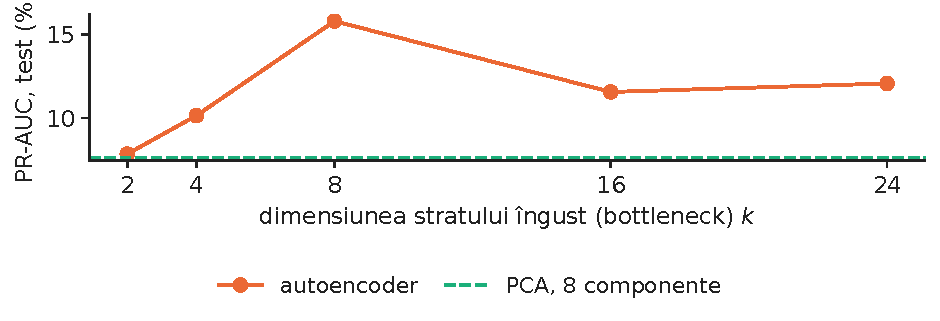
\includegraphics[width=\textwidth,height=0.391\textheight,keepaspectratio]{charts/ro/ae_bottleneck.pdf}\end{center}\vspace{-3mm}
\chartsource{Sursa: ULB Machine Learning Group și Worldline, tranzacții cu carduri (OpenML 1597). Date: estimări proprii; două zile din septembrie 2013; test = ultimele 20\,\% din interval.}
\vspace{0.5mm}
\begin{itemize}\setlength{\itemsep}{0pt}
  \item \textbf{PR-AUC după dimensiunea stratului îngust}: 7{,}8\,\% cu $k=2$, 15{,}8\,\% cu $k=8$, 12{,}1\,\% cu $k=24$ (media pe 2 semințe)
    \begin{itemize}\setlength{\itemsep}{0pt}
      \item Cel mai bun $k$ = 8
    \end{itemize}
  \item \textbf{Prea îngust}: chiar și plățile normale sînt reconstruite prost
    \begin{itemize}\setlength{\itemsep}{0pt}
      \item \textbf{prea larg}: rețeaua învață să copieze și fraudele
    \end{itemize}
\end{itemize}
\par\vfill\manager{alegeți $k$ pe o perioadă de validare, niciodată pe fraudele despre care veți raporta.}\par\vspace{0.5mm}
\par\vfill\noindent{\scriptsize\color{FooterGray}}\hfill\qlink{NN\_L8\_ae\_bottleneck}{Quantlets/L8/NN_L8_ae_bottleneck}\par\vspace{0.5mm}
\end{frame}

\begin{frame}{Fraudele identificate în primele 0,1\,\% dintre scoruri}
\footnotesize
\begin{columns}[T,onlytextwidth]
\begin{column}{0.52\textwidth}
{\scriptsize\renewcommand{\arraystretch}{1.3}\setlength{\tabcolsep}{4pt}
\begin{tabular}{@{}lrr@{}}\toprule
Detector & Fraude găsite & Pondere \\ \midrule
Autoencoder (fără etichete) & 8 & 10{,}7\,\% \\
PCA, 8 comp.\ (fără etichete) & 0 & 0{,}0\,\% \\
Regresie logistică (cu etichete) & 48 & 64{,}0\,\% \\
\bottomrule\end{tabular}}
\end{column}
\begin{column}{0.45\textwidth}
\begin{itemize}\setlength{\itemsep}{4pt}
  \item \textbf{Bugetul de alerte}
    \begin{itemize}\setlength{\itemsep}{0pt}
      \item 0,1\,\% dintre tranzacțiile de test = 57 de alerte de verificat
    \end{itemize}
  \item \textbf{Interpretare}
    \begin{itemize}\setlength{\itemsep}{0pt}
      \item Etichetele valorează mult: învățarea supervizată cîștigă ori de cîte ori există fraude confirmate
      \item Autoencoderul este detectorul necunoscutului, un complement, nu un înlocuitor
    \end{itemize}
\end{itemize}
\end{column}
\end{columns}
\par\vfill\manager{folosiți-le pe amîndouă: clasificatorul pentru tiparele cunoscute, autoencoderul pentru a scoate la iveală tipare noi, pe care investigatorii le etichetează.}\par\vspace{0.5mm}
\par\vfill\noindent{\scriptsize\color{FooterGray}(calcule proprii, partea de test, ponderat la datele complete)}\hfill\tryit{notebook, secțiunea 1}\par\vspace{0.5mm}
\end{frame}


\section{Autoencodere variaționale}

\begin{frame}{VAE transformă autoencoderul într-un generator probabilist}
\footnotesize
\intuition{În locul unui cod pentru fiecare intrare, codificatorul produce o distribuție; decodorul învață să transforme coduri aleatoare în date realiste.}
\begin{columns}[T,onlytextwidth]
\begin{column}{0.58\textwidth}
\[ \log p_{\btheta}(\mathbf x)\ \ge\ \underbrace{\E_{q_{\phi}(\mathbf z\mid\mathbf x)}\big[\log p_{\btheta}(\mathbf x\mid\mathbf z)\big]}_{\text{reconstrucție}}-\underbrace{\mathrm{KL}\big(q_{\phi}(\mathbf z\mid\mathbf x)\,\|\,p(\mathbf z)\big)}_{\text{regularizare}} \]{\footnotesize\begin{itemize}\setlength{\itemsep}{0pt}
  \item \textbf{\txtwhere}
    \begin{itemize}\setlength{\itemsep}{0pt}
      \item Membrul drept = marginea inferioară a verosimilității (ELBO)
      \item $q_\phi(\mathbf z\mid\mathbf x)=\mathcal N(\boldsymbol\mu_\phi(\mathbf x),\operatorname{diag}\boldsymbol\sigma^2_\phi(\mathbf x))$ = codificatorul
      \item $p_{\btheta}(\mathbf x\mid\mathbf z)$ = decodorul
      \item $p(\mathbf z)=\mathcal N(0,I)$ = distribuția a priori
      \item Al doilea termen este divergența Kullback--Leibler (KL).
    \end{itemize}
\end{itemize}\par}
\end{column}
\begin{column}{0.39\textwidth}
\begin{itemize}\setlength{\itemsep}{3pt}
  \item \textbf{De ce o margine}
    \begin{itemize}\setlength{\itemsep}{0pt}
      \item $\log p(\mathbf x)=\text{ELBO}+\mathrm{KL}\big(q(\mathbf z\mid\mathbf x)\|p(\mathbf z\mid\mathbf x)\big)$
      \item Diferența este eroarea codificatorului; derivarea, în Anexa A
    \end{itemize}
  \item \textbf{KL în formă închisă}
    \begin{itemize}\setlength{\itemsep}{0pt}
      \item $\mathrm{KL}=\tfrac12\sum_{j=1}^{k}\big(\mu_j^2+\sigma_j^2-\log\sigma_j^2-1\big)$
    \end{itemize}
\end{itemize}
\end{column}
\end{columns}
\par\vfill\manager{termenul KL face codurile aleatoare să aibă sens: aduce toate intrările în jurul originii spațiului latent.}\par\vspace{0.5mm}
\par\vfill\noindent{\scriptsize\color{FooterGray}(Kingma \& Welling, 2014; Bishop \& Bishop, 2024, sec.\ 19.2)}\hfill\tryit{notebook, secțiunea 2}\par\vspace{0.5mm}
\end{frame}

\begin{frame}{Trucul reparametrizării}
\footnotesize
\intuition{Extragerea aleatoare nu este derivabilă, dar o normală standard translatată și scalată este.}
\begin{columns}[T,onlytextwidth]
\begin{column}{0.58\textwidth}
\[ \mathbf z=\boldsymbol\mu_\phi(\mathbf x)+\boldsymbol\sigma_\phi(\mathbf x)\odot\boldsymbol\varepsilon,\qquad \boldsymbol\varepsilon\sim\mathcal N(0,I) \]\[ \nabla_\phi\,\E_{q_\phi}[h(\mathbf z)]=\E_{\boldsymbol\varepsilon}\big[\nabla_\phi\,h(\boldsymbol\mu_\phi+\boldsymbol\sigma_\phi\odot\boldsymbol\varepsilon)\big] \]{\footnotesize\begin{itemize}\setlength{\itemsep}{0pt}
  \item \textbf{\txtwhere}
    \begin{itemize}\setlength{\itemsep}{0pt}
      \item $\odot$ = produs element cu element
      \item Hazardul este în $\boldsymbol\varepsilon$, care nu depinde de $\phi$
      \item În practică ajunge o extragere a lui $\boldsymbol\varepsilon$ pentru fiecare imagine și pas.
    \end{itemize}
\end{itemize}\par}
\end{column}
\begin{column}{0.39\textwidth}
\begin{itemize}\setlength{\itemsep}{3pt}
  \item \textbf{VAE-ul nostru pe Fashion-MNIST}
    \begin{itemize}\setlength{\itemsep}{0pt}
      \item Imagini gri 28 $\times$ 28 cu 10 tipuri de îmbrăcăminte, înlocuitorul cifrelor MNIST
      \item 60\,000 de imagini de antrenare, 10\,000 de test; decodor Bernoulli (entropie încrucișată binară)
    \end{itemize}
  \item \textbf{Dimensiunea}
    \begin{itemize}\setlength{\itemsep}{0pt}
      \item 784 $\to$ 400 $\to$ 200 $\to$ $k$; 798\,816 de parametri pentru $k=16$; 20 de epoci
    \end{itemize}
\end{itemize}
\end{column}
\end{columns}
\par\vfill\manager{același truc stă la baza oricărui model care extrage aleator în interiorul rețelei: VAE, dropout ca inferență, politici stocastice.}\par\vspace{0.5mm}
\par\vfill\noindent{\scriptsize\color{FooterGray}(Kingma \& Welling, 2014; Xiao et al., 2017)}\hfill\tryit{notebook, secțiunea 2}\par\vspace{0.5mm}
\end{frame}

\begin{frame}{Un spațiu latent cu două dimensiuni separă tipurile de produse}
\small
\begin{center}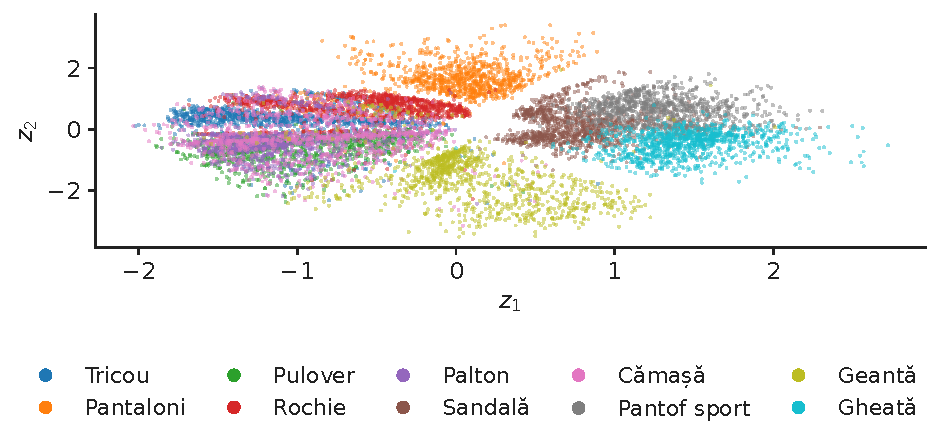
\includegraphics[width=\textwidth,height=0.580\textheight,keepaspectratio]{charts/ro/vae_latent.pdf}\end{center}\vspace{-3mm}
\chartsource{Sursa: Fashion-MNIST, Zalando Research (Xiao et al., 2017). Date: estimări proprii; 60.000 de imagini de antrenare și 10.000 de test.}
\vspace{0.5mm}
\begin{itemize}\setlength{\itemsep}{0pt}
  \item \textbf{Fără etichete}: VAE nu a văzut clasele, dar încălțămintea, gențile și hainele ocupă regiuni separate
  \item \textbf{Măsurat}: un clasificator cu 15 vecini pe cele două medii latente atinge o acuratețe de 71{,}7\,\% (5 partiții, imaginile de test)
\end{itemize}
\par\vfill\noindent{\scriptsize\color{FooterGray}}\hfill\qlink{NN\_L8\_vae\_latent}{Quantlets/L8/NN_L8_vae_latent}\par\vspace{0.5mm}
\end{frame}

\begin{frame}{Calitatea reconstrucțiilor VAE și a eșantioanelor generate}
\small
\begin{center}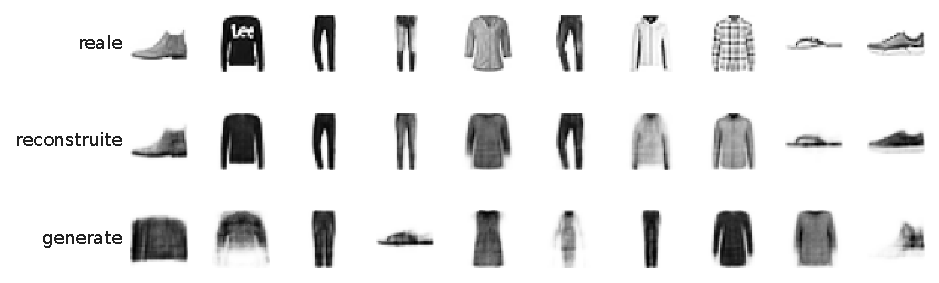
\includegraphics[width=\textwidth,height=0.480\textheight,keepaspectratio]{charts/ro/vae_samples.pdf}\end{center}\vspace{-3mm}
\chartsource{Sursa: Fashion-MNIST, Zalando Research (Xiao et al., 2017). Date: estimări proprii; 60.000 de imagini de antrenare și 10.000 de test.}
\vspace{0.5mm}
\begin{itemize}\setlength{\itemsep}{0pt}
  \item \textbf{Rîndurile}: imagini reale de test
    \begin{itemize}\setlength{\itemsep}{0pt}
      \item Reconstrucția lor printr-un cod cu 16 dimensiuni
      \item Imagini noi decodate din coduri aleatoare $\mathbf z\sim\mathcal N(0,I)$
    \end{itemize}
  \item \textbf{Neclaritatea} vine din distribuția a posteriori gaussiană și din pierderea calculată pixel cu pixel: decodorul face media detaliilor plauzibile
\end{itemize}
\par\vfill\noindent{\scriptsize\color{FooterGray}}\hfill\qlink{NN\_L8\_vae\_samples}{Quantlets/L8/NN_L8_vae_samples}\par\vspace{0.5mm}
\end{frame}

\begin{frame}{Compromisul dintre reconstrucție și penalizarea KL în timpul antrenării}
\small
\begin{center}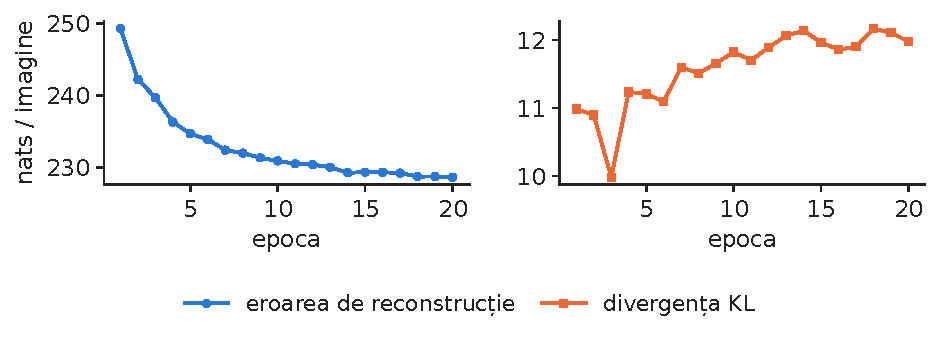
\includegraphics[width=\textwidth,height=0.480\textheight,keepaspectratio]{charts/ro/vae_elbo.pdf}\end{center}\vspace{-3mm}
\chartsource{Sursa: Fashion-MNIST, Zalando Research (Xiao et al., 2017). Date: estimări proprii; 60.000 de imagini de antrenare și 10.000 de test.}
\vspace{0.5mm}
\begin{itemize}\setlength{\itemsep}{0pt}
  \item \textbf{Test, $k=16$, ultima epocă}: reconstrucția 228{,}6 nats pe imagine, KL 12{,}0 nats
    \begin{itemize}\setlength{\itemsep}{0pt}
      \item ELBO \ensuremath{-}240{,}6 nats
    \end{itemize}
  \item \textbf{KL crește} cînd eroarea scade: codificatorul folosește mai multă informație pentru fiecare imagine pe măsură ce învață
\end{itemize}
\par\vfill\noindent{\scriptsize\color{FooterGray}(calcule proprii, sămînța 1)}\hfill\qlink{NN\_L8\_vae\_elbo}{Quantlets/L8/NN_L8_vae_elbo}\par\vspace{0.5mm}
\end{frame}

\begin{frame}{$\beta$-VAE: calitatea reconstrucției și structura spațiului latent}
\footnotesize
\begin{columns}[T,onlytextwidth]
\begin{column}{0.50\textwidth}
\[ \loss_\beta=-\E_{q}[\log p(\mathbf x\mid\mathbf z)]+\beta\,\mathrm{KL}\big(q(\mathbf z\mid\mathbf x)\|p(\mathbf z)\big) \]{\scriptsize\renewcommand{\arraystretch}{1.3}\setlength{\tabcolsep}{4pt}
\begin{tabular}{@{}lrrr@{}}\toprule
$\beta$ & Reconstrucție & KL & Dim.\ active \\ \midrule
0{,}5 & 222{,}5 & 17{,}8 & 9 \\
1{,}0 & 228{,}6 & 12{,}0 & 6 \\
4{,}0 & 242{,}5 & 6{,}4 & 4 \\
\bottomrule\end{tabular}}
\end{column}
\begin{column}{0.47\textwidth}
\begin{itemize}\setlength{\itemsep}{4pt}
  \item \textbf{$\beta$ mai mare}
    \begin{itemize}\setlength{\itemsep}{0pt}
      \item Mai puține dimensiuni latente active (KL pe dimensiune $>0{,}05$): de la 9 la 4 din 16
      \item Reconstrucție mai slabă, coduri mai netede și mai separate
    \end{itemize}
  \item \textbf{$\beta$ mai mic}
    \begin{itemize}\setlength{\itemsep}{0pt}
      \item Mai aproape de un autoencoder simplu: copii bune, eșantioane slabe
    \end{itemize}
\end{itemize}
\end{column}
\end{columns}
\par\vfill\manager{pentru generarea de scenarii preferați un spațiu latent ordonat ($\beta\ge1$)
    \begin{itemize}\setlength{\itemsep}{0pt}
      \item Pentru comprimare, reconstrucția ($\beta<1$).
    \end{itemize}}\par\vspace{0.5mm}
\par\vfill\noindent{\scriptsize\color{FooterGray}(Higgins et al., 2017; calcule proprii, imaginile de test, 20 de epoci)}\hfill\tryit{notebook, secțiunea 2}\par\vspace{0.5mm}
\end{frame}


\section{Rețele generative adversariale}

\begin{frame}{Rețelele generative adversariale: generatorul și discriminatorul}
\footnotesize
\intuition{Generatorul face date false din zgomot, discriminatorul caută falsul; fiecare progresează împotriva celuilalt.}
\begin{columns}[T,onlytextwidth]
\begin{column}{0.58\textwidth}
\[ \min_{G}\max_{D}\ \E_{\mathbf x\sim p_{data}}\big[\log D(\mathbf x)\big]+\E_{\mathbf z\sim p(\mathbf z)}\big[\log\big(1-D(G(\mathbf z))\big)\big] \]\[ D^{*}(\mathbf x)=\frac{p_{data}(\mathbf x)}{p_{data}(\mathbf x)+p_G(\mathbf x)}\ \Rightarrow\ \text{valoarea}=-\log4+2\,\mathrm{JS}(p_{data}\|p_G) \]{\footnotesize\begin{itemize}\setlength{\itemsep}{0pt}
  \item \textbf{\txtwhere}
    \begin{itemize}\setlength{\itemsep}{0pt}
      \item $G$ = rețeaua generator, $D$ = discriminatorul (probabilitatea ca $\mathbf x$ să fie real)
      \item $p_G$ = distribuția lui $G(\mathbf z)$
      \item Divergența Jensen--Shannon (JS), nulă numai cînd $p_G=p_{data}$.
    \end{itemize}
\end{itemize}\par}
\end{column}
\begin{column}{0.39\textwidth}
\begin{itemize}\setlength{\itemsep}{3pt}
  \item \textbf{La echilibru}
    \begin{itemize}\setlength{\itemsep}{0pt}
      \item $D^{*}=1/2$ peste tot: detectivul doar ghicește; pierderea discriminatorului $2\log 2$
    \end{itemize}
  \item \textbf{Fără verosimilitate}
    \begin{itemize}\setlength{\itemsep}{0pt}
      \item Un GAN nu scrie niciodată $p_G$; doar învață să extragă din ea
    \end{itemize}
\end{itemize}
\end{column}
\end{columns}
\par\vfill\manager{un GAN se judecă după eșantioane (cozi, dependență), nu după verosimilitate.}\par\vspace{0.5mm}
\par\vfill\noindent{\scriptsize\color{FooterGray}(Goodfellow et al., 2014; Bishop \& Bishop, 2024, ch.\ 17)}\hfill\tryit{notebook, secțiunea 3}\par\vspace{0.5mm}
\end{frame}

\begin{frame}{Antrenarea unui GAN: pași alternativi și pierderea nesaturată}
\footnotesize
\intuition{La fiecare pas se actualizează întîi detectivul, apoi falsificatorul.}
\begin{columns}[T,onlytextwidth]
\begin{column}{0.58\textwidth}
\[ \loss_D=-\tfrac1m\sum_{i}\big[\log D(\mathbf x_i)+\log(1-D(G(\mathbf z_i)))\big] \]\[ \loss_G=-\tfrac1m\sum_{i}\log D(G(\mathbf z_i))\quad\text{(nesaturată)} \]{\footnotesize\begin{itemize}\setlength{\itemsep}{0pt}
  \item \textbf{\txtwhere}
    \begin{itemize}\setlength{\itemsep}{0pt}
      \item $m=256$ de zile pe lot
      \item $\mathbf z\in\R^8$ normal standard
      \item $\loss_G$ evită gradientul nul al lui $\log(1-D(G))$ cînd $D$ cîștigă devreme
      \item Adam, rata $2\cdot10^{-4}$, $\beta_1=0{,}5$.
    \end{itemize}
\end{itemize}\par}
\end{column}
\begin{column}{0.39\textwidth}
\begin{itemize}\setlength{\itemsep}{3pt}
  \item \textbf{GAN-ul nostru}
    \begin{itemize}\setlength{\itemsep}{0pt}
      \item Randamentele logaritmice zilnice ale indicelui S\&P 500, 4 ianuarie 2005 -- 2019, 3\,774 de zile, standardizate
      \item Generator cu 4\,801 de parametri, discriminator cu 4\,353; 6\,000 de pași, 3 semințe
    \end{itemize}
\end{itemize}
\end{column}
\end{columns}
\par\vfill\manager{o pierdere a discriminatorului blocată la zero arată că generatorul nu mai învață.}\par\vspace{0.5mm}
\par\vfill\noindent{\scriptsize\color{FooterGray}(Goodfellow et al., 2014)}\hfill\tryit{notebook, secțiunea 3}\par\vspace{0.5mm}
\end{frame}

\begin{frame}{Cele două pierderi se stabilizează lîngă valorile de echilibru}
\small
\begin{center}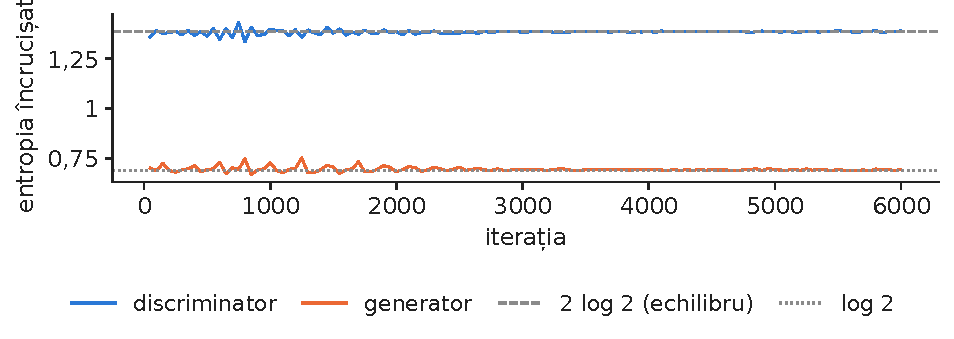
\includegraphics[width=\textwidth,height=0.500\textheight,keepaspectratio]{charts/ro/gan_losses.pdf}\end{center}\vspace{-3mm}
\chartsource{Sursa: Yahoo Finance, cotații zilnice. Date: estimări proprii; S\&P 500 4 ianuarie 2005 - 31 decembrie 2019, zile de tranzacționare.}
\vspace{0.5mm}
\begin{itemize}\setlength{\itemsep}{0pt}
  \item \textbf{Echilibrul}: pierderea discriminatorului oscilează în jurul lui $2\log2$, iar a generatorului în jurul lui $\log 2$, valorile lui $D^{*}=1/2$
  \item \textbf{Nicio garanție de convergență}: jocul pe gradienți poate oscila
    \begin{itemize}\setlength{\itemsep}{0pt}
      \item Curbele de pierdere nu măsoară calitatea eșantioanelor
    \end{itemize}
\end{itemize}
\par\vfill\noindent{\scriptsize\color{FooterGray}}\hfill\qlink{NN\_L8\_gan\_losses}{Quantlets/L8/NN_L8_gan_losses}\par\vspace{0.5mm}
\end{frame}

\begin{frame}{GAN-ul reproduce cozile groase pe care modelul gaussian nu le surprinde}
\small
\begin{center}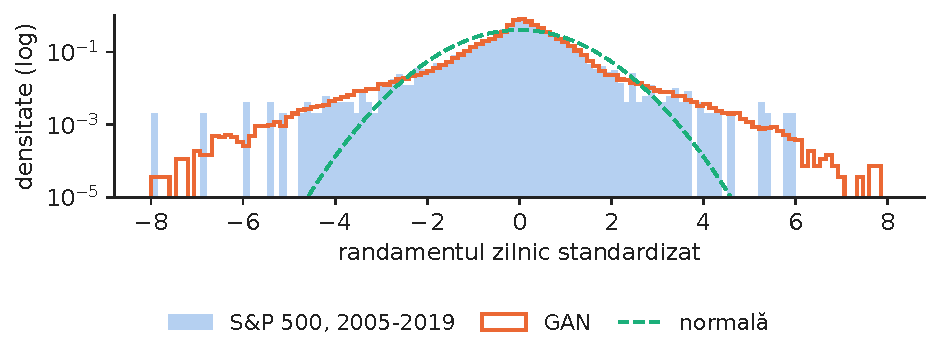
\includegraphics[width=\textwidth,height=0.520\textheight,keepaspectratio]{charts/ro/gan_density.pdf}\end{center}\vspace{-3mm}
\chartsource{Sursa: Yahoo Finance, cotații zilnice. Date: estimări proprii; S\&P 500 4 ianuarie 2005 - 31 decembrie 2019, zile de tranzacționare.}
\vspace{0.5mm}
\begin{itemize}\setlength{\itemsep}{0pt}
  \item \textbf{Excesul de aplatizare}: real 11{,}86, GAN 6{,}65 (abatere standard 0{,}48 pe 3 semințe), normala 0
  \item \textbf{Distanța Kolmogorov--Smirnov} față de randamentele reale: GAN 0{,}030, normala estimată 0{,}115
\end{itemize}
\par\vfill\noindent{\scriptsize\color{FooterGray}(Cont, 2001)}\hfill\qlink{NN\_L8\_gan\_density}{Quantlets/L8/NN_L8_gan_density}\par\vspace{0.5mm}
\end{frame}

\begin{frame}{Un test de risc: valoarea la risc de 1\,\% în anii de după antrenare}
\footnotesize
\begin{columns}[T,onlytextwidth]
\begin{column}{0.52\textwidth}
\[ \mathrm{VaR}_{0.01}=-q_{0.01}(r),\qquad \hat\pi=\frac{1}{T}\sum_{t=1}^{T}\mathbf 1\{r_t<q_{0.01}\} \]{\scriptsize\renewcommand{\arraystretch}{1.3}\setlength{\tabcolsep}{4pt}
\begin{tabular}{@{}lrr@{}}\toprule
Metoda (estimată 2005--2019) & Cuantila de 1\,\% & Depășiri \\ \midrule
Simulare istorică & \ensuremath{-}3{,}48\,\% & 1{,}11\,\% \\
Eșantioane GAN (3 semințe) & \ensuremath{-}3{,}61\,\% & 0{,}95\,\% \\
Normală & \ensuremath{-}2{,}67\,\% & 2{,}39\,\% \\
\bottomrule\end{tabular}}
\end{column}
\begin{column}{0.45\textwidth}
\begin{itemize}\setlength{\itemsep}{4pt}
  \item \textbf{Perioada de test}
    \begin{itemize}\setlength{\itemsep}{0pt}
      \item 2 ianuarie 2020 -- 30 octombrie 2026, 1\,717 de zile; o valoare VaR corectă de 1\,\% este depășită în circa 17 zile
    \end{itemize}
  \item \textbf{Interpretare}
    \begin{itemize}\setlength{\itemsep}{0pt}
      \item Cuantila GAN este la fel de bună ca simularea istorică; normala este depășită în 2{,}39\,\% dintre zile
      \item Numai cuantile necondiționate: niciun model de aici nu reacționează la volatilitate
      \item Pierderea așteptată în coadă (ES), media pierderilor dincolo de VaR, depinde de aceeași coadă
    \end{itemize}
\end{itemize}
\end{column}
\end{columns}
\par\vfill\manager{un generator este atît de bun cît măsura de risc pe care o reproduce: testați-l retrospectiv ca pe orice model VaR (Kupiec, 1995).}\par\vspace{0.5mm}
\par\vfill\noindent{\scriptsize\color{FooterGray}(calcule proprii)}\hfill\tryit{notebook, secțiunea 3}\par\vspace{0.5mm}
\end{frame}

\begin{frame}{Un GAN pe zile izolate nu poate învăța gruparea volatilității}
\small
\begin{center}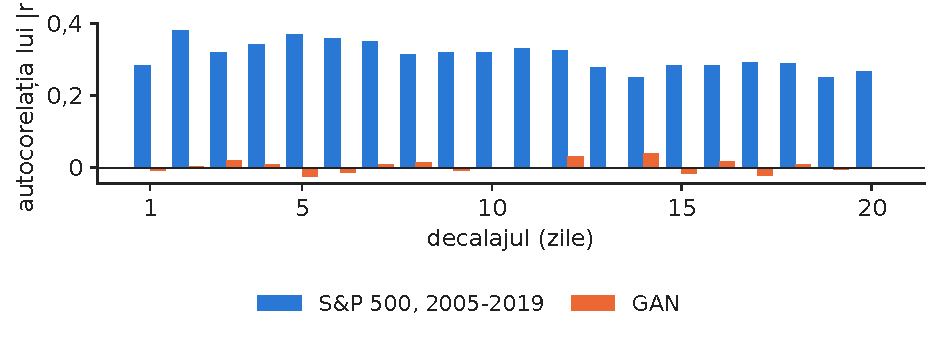
\includegraphics[width=\textwidth,height=0.480\textheight,keepaspectratio]{charts/ro/gan_acf.pdf}\end{center}\vspace{-3mm}
\chartsource{Sursa: Yahoo Finance, cotații zilnice. Date: estimări proprii; S\&P 500 4 ianuarie 2005 - 31 decembrie 2019, zile de tranzacționare.}
\vspace{0.5mm}
\begin{itemize}\setlength{\itemsep}{0pt}
  \item \textbf{Randamentele reale}: autocorelația lui $|r_t|$ este 0{,}28 la decalajul 1 și încă 0{,}27 la decalajul 20: perioadele calme și cele agitate se grupează
  \item \textbf{Eșantioanele GAN} sînt extrageri independente (\ensuremath{-}0{,}01 la decalajul 1): distribuția marginală corectă, dinamica greșită
    \begin{itemize}\setlength{\itemsep}{0pt}
      \item Modelele de secvențe (TimeGAN, Quant GANs) generează traiectorii întregi
    \end{itemize}
\end{itemize}
\par\vfill\noindent{\scriptsize\color{FooterGray}(Cont, 2001; Yoon et al., 2019; Wiese et al., 2020)}\hfill\qlink{NN\_L8\_gan\_acf}{Quantlets/L8/NN_L8_gan_acf}\par\vspace{0.5mm}
\end{frame}

\begin{frame}{Colapsul modurilor și GAN-ul Wasserstein}
\footnotesize
\intuition{Un generator poate cîștiga producînd cîteva eșantioane convingătoare; distanța Wasserstein dă gradienți utili chiar cînd suporturile nu se suprapun.}
\begin{columns}[T,onlytextwidth]
\begin{column}{0.58\textwidth}
\[ W_1(p_{data},p_G)=\sup_{\|f\|_{L}\le1}\ \E_{p_{data}}[f(\mathbf x)]-\E_{p_G}[f(\mathbf x)] \]{\footnotesize\begin{itemize}\setlength{\itemsep}{0pt}
  \item \textbf{\txtwhere}
    \begin{itemize}\setlength{\itemsep}{0pt}
      \item $f$ = rețeaua critic, constrînsă să fie 1-Lipschitz (tăierea ponderilor sau o penalizare a gradientului)
      \item Generatorul minimizează $W_1$: GAN-ul Wasserstein (WGAN).
    \end{itemize}
\end{itemize}\par}
\end{column}
\begin{column}{0.39\textwidth}
\begin{itemize}\setlength{\itemsep}{3pt}
  \item \textbf{Colapsul modurilor}
    \begin{itemize}\setlength{\itemsep}{0pt}
      \item Generatorul duce toți $\mathbf z$ în aceeași regiune: de exemplu, numai zile calme, niciodată prăbușiri
    \end{itemize}
  \item \textbf{Verificări}
    \begin{itemize}\setlength{\itemsep}{0pt}
      \item Comparați cuantilele din coadă, ponderea zilelor extreme și dispersia eșantioanelor cu datele reale
    \end{itemize}
\end{itemize}
\end{column}
\end{columns}
\par\vfill\manager{un generator pentru teste de stres care a colapsat pe zilele calme este mai rău decît lipsa unui generator.}\par\vspace{0.5mm}
\par\vfill\noindent{\scriptsize\color{FooterGray}(Arjovsky, Chintala \& Bottou, 2017)}\par\vspace{0.5mm}
\end{frame}


\section{Modele de difuzie}

\begin{frame}{Modelele de difuzie: adăugarea și eliminarea treptată a zgomotului}
\footnotesize
\intuition{Cu zgomot gaussian adăugat treptat, orice date devin zgomot pur; o rețea învață fiecare pas înapoi.}
\begin{columns}[T,onlytextwidth]
\begin{column}{0.58\textwidth}
\[ q(\mathbf x_t\mid\mathbf x_{t-1})=\mathcal N\big(\sqrt{1-\beta_t}\,\mathbf x_{t-1},\ \beta_tI\big) \]\[ q(\mathbf x_t\mid\mathbf x_0)=\mathcal N\big(\sqrt{\bar\alpha_t}\,\mathbf x_0,\ (1-\bar\alpha_t)I\big),\quad \bar\alpha_t=\prod_{s=1}^{t}(1-\beta_s) \]{\footnotesize\begin{itemize}\setlength{\itemsep}{0pt}
  \item \textbf{\txtwhere}
    \begin{itemize}\setlength{\itemsep}{0pt}
      \item $\mathbf x_0$ = o observație reală (aici o curbă a randamentelor standardizată)
      \item $\beta_t$ = programul zgomotului, liniar de la $10^{-4}$ la 0,02 în $T$ = 200 de pași
      \item $\bar\alpha_T\approx0$, deci $\mathbf x_T$ este aproape normal standard.
    \end{itemize}
\end{itemize}\par}
\end{column}
\begin{column}{0.39\textwidth}
\begin{itemize}\setlength{\itemsep}{3pt}
  \item \textbf{Formă închisă}
    \begin{itemize}\setlength{\itemsep}{0pt}
      \item Orice pas $t$ se obține dintr-o singură extragere: $\mathbf x_t=\sqrt{\bar\alpha_t}\mathbf x_0+\sqrt{1-\bar\alpha_t}\,\boldsymbol\varepsilon$
    \end{itemize}
  \item \textbf{Fără parametri}
    \begin{itemize}\setlength{\itemsep}{0pt}
      \item Procesul înainte este fix; numai procesul invers se învață
    \end{itemize}
\end{itemize}
\end{column}
\end{columns}
\par\vfill\manager{difuzia transformă generarea în multe probleme mici de regresie
    \begin{itemize}\setlength{\itemsep}{0pt}
      \item De aceea se antrenează stabil.
    \end{itemize}}\par\vspace{0.5mm}
\par\vfill\noindent{\scriptsize\color{FooterGray}(Sohl-Dickstein et al., 2015; Ho, Jain \& Abbeel, 2020)}\hfill\tryit{notebook, secțiunea 4}\par\vspace{0.5mm}
\end{frame}

\begin{frame}{Procesul înainte pe o curbă reală a randamentelor}
\small
\begin{center}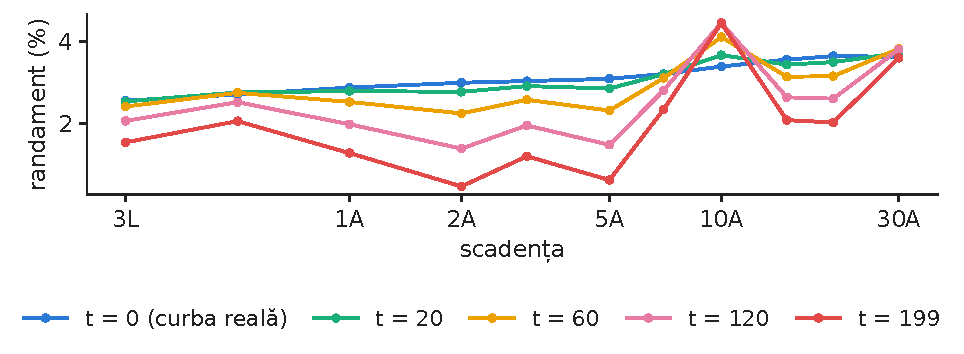
\includegraphics[width=\textwidth,height=0.520\textheight,keepaspectratio]{charts/ro/diffusion_forward.pdf}\end{center}\vspace{-3mm}
\chartsource{Sursa: Banca Centrală Europeană, curba randamentelor AAA din zona euro. Date: curba din 30 octombrie 2026; programul de zgomot din curs (mecanism).}
\vspace{0.5mm}
\begin{itemize}\setlength{\itemsep}{0pt}
  \item \textbf{Curba din 30 octombrie 2026}, 11 scadențe, de la 3 luni la 30 de ani
    \begin{itemize}\setlength{\itemsep}{0pt}
      \item La $t=199$ forma a dispărut și a rămas doar zgomot
    \end{itemize}
  \item \textbf{Rețeaua} trebuie să învețe drumul înapoi, de la dreapta la stînga, cîte un pas mic
\end{itemize}
\par\vfill\noindent{\scriptsize\color{FooterGray}(mecanism ilustrat pe date reale; o singură extragere a zgomotului)}\hfill\qlink{NN\_L8\_diffusion\_forward}{Quantlets/L8/NN_L8_diffusion_forward}\par\vspace{0.5mm}
\end{frame}

\begin{frame}{Învățarea eliminării zgomotului: prezicem zgomotul adăugat}
\footnotesize
\intuition{Rețeaua vede curba cu zgomot și pasul $t$ și ghicește zgomotul; scăzîndu-l pas cu pas, obținem o curbă nouă.}
\begin{columns}[T,onlytextwidth]
\begin{column}{0.58\textwidth}
\[ \loss(\btheta)=\E_{t,\mathbf x_0,\boldsymbol\varepsilon}\Big\|\boldsymbol\varepsilon-\boldsymbol\varepsilon_{\btheta}\big(\sqrt{\bar\alpha_t}\mathbf x_0+\sqrt{1-\bar\alpha_t}\,\boldsymbol\varepsilon,\ t\big)\Big\|^2 \]\[ \mathbf x_{t-1}=\frac{1}{\sqrt{\alpha_t}}\Big(\mathbf x_t-\frac{\beta_t}{\sqrt{1-\bar\alpha_t}}\boldsymbol\varepsilon_{\btheta}(\mathbf x_t,t)\Big)+\sqrt{\beta_t}\,\mathbf u,\ \ \mathbf u\sim\mathcal N(0,I) \]{\footnotesize\begin{itemize}\setlength{\itemsep}{0pt}
  \item \textbf{\txtwhere}
    \begin{itemize}\setlength{\itemsep}{0pt}
      \item $\boldsymbol\varepsilon_{\btheta}$ = rețeaua care elimină zgomotul
      \item $\alpha_t=1-\beta_t$
      \item $t$ uniform pe $\{1,\dots,T\}$
      \item Pierderea este un ELBO simplificat și reponderat.
    \end{itemize}
\end{itemize}\par}
\end{column}
\begin{column}{0.39\textwidth}
\begin{itemize}\setlength{\itemsep}{3pt}
  \item \textbf{Rețeaua noastră}
    \begin{itemize}\setlength{\itemsep}{0pt}
      \item MLP cu 3 straturi ascunse de 256 și o reprezentare sinusoidală a lui $t$: 145\,675 de parametri
      \item 12\,000 de pași cu loturi de 512 curbe; 5.000 de curbe generate pe sămînță
    \end{itemize}
  \item \textbf{Date}
    \begin{itemize}\setlength{\itemsep}{0pt}
      \item 5\,664 de curbe zilnice ale Băncii Centrale Europene, 6 septembrie 2004 -- 30 octombrie 2026
    \end{itemize}
\end{itemize}
\end{column}
\end{columns}
\par\vfill\manager{aceeași pierdere stă la baza generatoarelor de imagini, iar aici generează scenarii de dobîndă.}\par\vspace{0.5mm}
\par\vfill\noindent{\scriptsize\color{FooterGray}(Ho, Jain \& Abbeel, 2020; Bishop \& Bishop, 2024, ch.\ 20)}\hfill\tryit{notebook, secțiunea 4}\par\vspace{0.5mm}
\end{frame}

\begin{frame}{Cele două regimuri ale dobînzilor euro în eșantioanele generate prin difuzie și de modelul gaussian}
\small
\begin{center}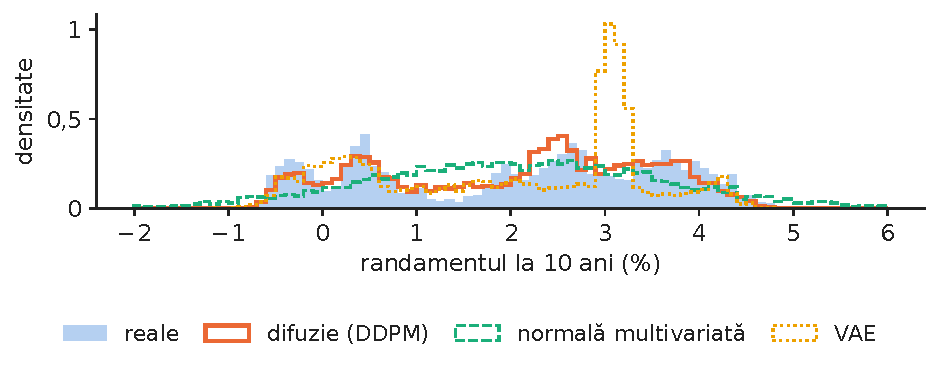
\includegraphics[width=\textwidth,height=0.427\textheight,keepaspectratio]{charts/ro/yc_density.pdf}\end{center}\vspace{-3mm}
\chartsource{Sursa: Banca Centrală Europeană, curba randamentelor AAA din zona euro. Date: estimări proprii; 6 septembrie 2004 - 30 octombrie 2026, zile lucrătoare.}
\vspace{0.5mm}
\begin{itemize}\setlength{\itemsep}{0pt}
  \item \textbf{Randamentul real la 10 ani}: de la \ensuremath{-}0{,}82\,\% la 4{,}78\,\%, negativ în 13{,}8\,\% dintre zile: un regim de dobînzi scăzute și unul de dobînzi normale
  \item \textbf{Distanța Wasserstein} dintre randamentul generat la 10 ani și cel real: DDPM 0{,}149, VAE 0{,}191, normala 0{,}325 puncte procentuale
\end{itemize}
\par\vfill\noindent{\scriptsize\color{FooterGray}}\hfill\qlink{NN\_L8\_yc\_density}{Quantlets/L8/NN_L8_yc_density}\par\vspace{0.5mm}
\end{frame}

\begin{frame}{Difuzia păstrează dependența neliniară dintre nivel și pantă}
\small
\begin{center}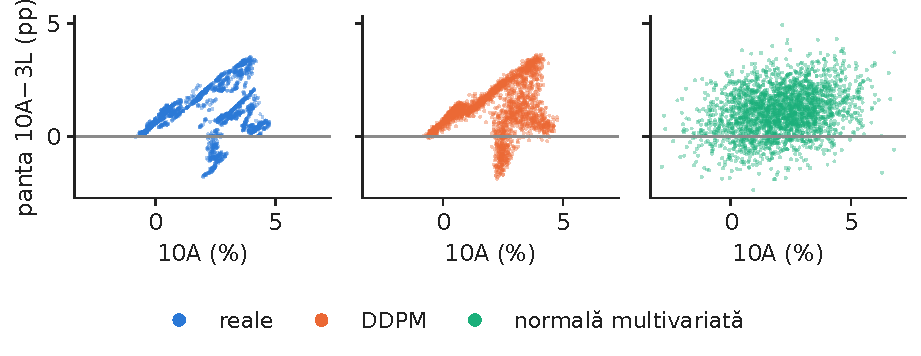
\includegraphics[width=\textwidth,height=0.500\textheight,keepaspectratio]{charts/ro/yc_scatter.pdf}\end{center}\vspace{-3mm}
\chartsource{Sursa: Banca Centrală Europeană, curba randamentelor AAA din zona euro. Date: estimări proprii; 6 septembrie 2004 - 30 octombrie 2026, zile lucrătoare.}
\vspace{0.5mm}
\begin{itemize}\setlength{\itemsep}{0pt}
  \item \textbf{Curbe inversate} (10 ani sub 3 luni): 8{,}7\,\% dintre zilele reale, 10{,}2\,\% dintre eșantioanele difuziei, 14{,}7\,\% dintre cele normale
  \item \textbf{Distanța pantei} (Wasserstein): DDPM 0{,}099, VAE 0{,}242, normala 0{,}113
\end{itemize}
\par\vfill\noindent{\scriptsize\color{FooterGray}}\hfill\qlink{NN\_L8\_yc\_scatter}{Quantlets/L8/NN_L8_yc_scatter}\par\vspace{0.5mm}
\end{frame}

\begin{frame}{Un VAE cu doi factori ai curbei redescoperă nivelul și panta}
\small
\begin{center}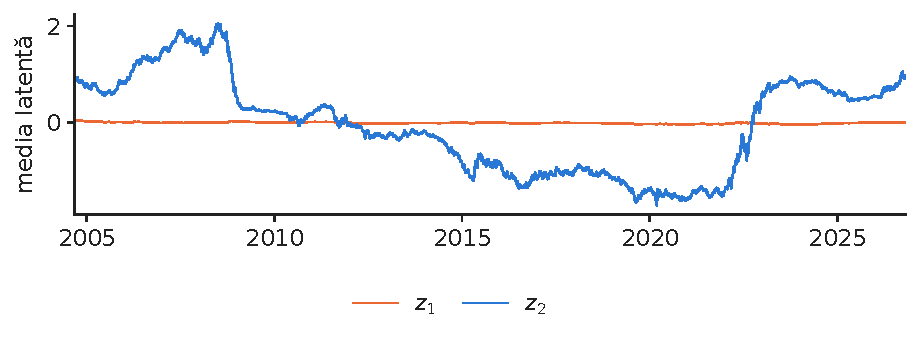
\includegraphics[width=\textwidth,height=0.480\textheight,keepaspectratio]{charts/ro/yc_latent_time.pdf}\end{center}\vspace{-3mm}
\chartsource{Sursa: Banca Centrală Europeană, curba randamentelor AAA din zona euro. Date: estimări proprii; 6 septembrie 2004 - 30 octombrie 2026, zile lucrătoare.}
\vspace{0.5mm}
\begin{itemize}\setlength{\itemsep}{0pt}
  \item \textbf{Corelațiile} mediilor latente cu nivelul (media celor 11 randamente) și cu panta (10 ani minus 3 luni): pînă la 0{,}99 și 0{,}66 în valoare absolută
  \item \textbf{Comprimare interpretabilă}: traiectoria latentă urmărește perioada de dobînzi scăzute 2014--2021 și înăsprirea din 2022, fără să i se spună
\end{itemize}
\par\vfill\noindent{\scriptsize\color{FooterGray}(Svensson, 1994)}\hfill\qlink{NN\_L8\_yc\_latent\_time}{Quantlets/L8/NN_L8_yc_latent_time}\par\vspace{0.5mm}
\end{frame}


\section{Modelele generative în practică}

\begin{frame}{Criterii de evaluare a datelor financiare sintetice}
\footnotesize
\begin{columns}[T,onlytextwidth]
\begin{column}{0.49\textwidth}
\begin{itemize}\setlength{\itemsep}{5pt}
  \item \textbf{Fidelitatea}
    \begin{itemize}\setlength{\itemsep}{0pt}
      \item Distribuțiile marginale și cozile (aplatizarea, cuantila de 1\,\%), dependența între active și în timp (autocorelația lui $|r_t|$)
    \end{itemize}
  \item \textbf{Diversitatea}
    \begin{itemize}\setlength{\itemsep}{0pt}
      \item Fără colaps al modurilor: ponderea zilelor extreme și a regimurilor ca în date
    \end{itemize}
  \item \textbf{Utilitatea}
    \begin{itemize}\setlength{\itemsep}{0pt}
      \item Antrenare pe date sintetice, test pe date reale (TSTR): un model estimat pe date sintetice trebuie să funcționeze pe date reale
    \end{itemize}
\end{itemize}
\end{column}
\begin{column}{0.48\textwidth}
\begin{itemize}\setlength{\itemsep}{5pt}
  \item \textbf{Confidențialitatea}
    \begin{itemize}\setlength{\itemsep}{0pt}
      \item Generatoarele pot memora înregistrări: verificați distanța fiecărui eșantion pînă la cea mai apropiată înregistrare reală
    \end{itemize}
  \item \textbf{Fișa noastră de evaluare}
    \begin{itemize}\setlength{\itemsep}{0pt}
      \item Randamentele GAN: cozile corecte, gruparea volatilității greșită
      \item Curbele DDPM: regimurile și inversările corecte, normala greșită
    \end{itemize}
\end{itemize}
\end{column}
\end{columns}
\par\vfill\manager{nu folosiți date sintetice într-o decizie înainte ca ele să treacă aceleași teste retrospective ca modelul pe care îl alimentează.}\par\vspace{0.5mm}
\par\vfill\noindent{\scriptsize\color{FooterGray}(Cont, 2001; Yoon et al., 2019)}\par\vspace{0.5mm}
\end{frame}

\begin{frame}{Alegerea unui model generativ}
\footnotesize
{\scriptsize\renewcommand{\arraystretch}{1.25}\setlength{\tabcolsep}{4pt}
\begin{tabular}{@{}p{0.22\textwidth}p{0.17\textwidth}p{0.17\textwidth}p{0.17\textwidth}p{0.17\textwidth}@{}}\toprule
Nevoia & AE & VAE & GAN & DDPM \\ \midrule
Scor de anomalie & da (eroarea) & da (ELBO) & indirect & da (marginea) \\
Calitatea eșantioanelor & -- & neclare & clare & cea mai bună \\
Viteza generării & -- & o trecere & o trecere & 200 de treceri \\
Stabilitatea antrenării & mare & mare & mică & mare \\
Factori latenți & da & da, netezi & fără invers & nu \\
\bottomrule\end{tabular}}
\vspace{2mm}
\begin{itemize}\setlength{\itemsep}{2pt}
  \item \textbf{Regulă practică}: autoencodere pentru monitorizare, VAE pentru comprimare și explorare, difuzie pentru simulări fidele, GAN cînd generarea trebuie să fie rapidă
\end{itemize}
\par\vfill\noindent{\scriptsize\color{FooterGray}(Bishop \& Bishop, 2024, ch.\ 16--20)}\par\vspace{0.5mm}
\end{frame}


\section{Concluzii}

\begin{frame}{Idei principale}
\small
\begin{itemize}\setlength{\itemsep}{6pt}
  \item \textbf{Autoencoderele} modelează ``normalul'': la fraudele cu carduri, PR-AUC 14{,}2\,\% fără etichete, față de 80{,}4\,\% pentru un clasificator cu etichete
  \item \textbf{VAE} maximizează ELBO = reconstrucție $-$ KL
    \begin{itemize}\setlength{\itemsep}{0pt}
      \item Trucul reparametrizării le face antrenabile
      \item $\beta$ schimbă detaliul pe un spațiu latent ordonat
    \end{itemize}
  \item \textbf{GAN} reproduc cozile groase (aplatizare 6{,}65, față de 11{,}86 real) și o valoare VaR de 1\,\% utilizabilă, dar nu și gruparea volatilității cînd sînt antrenate pe zile izolate
  \item \textbf{Difuzia} învață să elimine zgomotul
    \begin{itemize}\setlength{\itemsep}{0pt}
      \item Pe curbele euro păstrează ambele regimuri de dobîndă și inversările pe care distribuția normală nu le vede
    \end{itemize}
\end{itemize}
\end{frame}

\begin{frame}{Cercetările grupului nostru: modele generative pentru riscul extrem}
\footnotesize
\begin{itemize}\setlength{\itemsep}{5pt}
  \item \textbf{Modele mari de limbaj (LLM) ca instrumente de prognoză a riscului: LLM-VaR și LLM-ES} (Pele, Bolovăneanu, Lin, Ren, Ginavar, Spilak, Andrei, Toma, Lessmann \& Härdle, 2026)
    \begin{itemize}\setlength{\itemsep}{0pt}
      \item Lucrarea folosește modele de limbaj generative, cărora li se dau istoricele randamentelor, pentru prognoza valorii la risc și a pierderii așteptate în coadă, evaluate cu testele retrospective standard
    \end{itemize}
  \item \textbf{Modele fundaționale pentru riscul extrem} (Jheng, Tak, Găman, Mazurencu-Marinescu-Pele \& Pele, 2026)
    \begin{itemize}\setlength{\itemsep}{0pt}
      \item Lucrarea folosește modele probabiliste de prognoză preantrenate, care generează traiectorii, fără reantrenare și cu calibrare conformală, pentru prognoza VaR și ES pe piețele din Europa Centrală și de Est
    \end{itemize}
  \item \textbf{Legătura cu acest curs}: ambele lucrări tratează un generator de scenarii ca pe un model de risc și îl judecă prin testele retrospective folosite aici pentru GAN
\end{itemize}
\vspace{1mm}{\scriptsize Rezultatele de pe acest slide sînt cele din lucrări; cifrele de pe celelalte slide-uri provin din calculele noastre.}
\par\vfill\noindent{\scriptsize\color{FooterGray}(Academia de Studii Economice din București; Academia Română, Institutul de Prognoză Economică)}\par\vspace{0.5mm}
\end{frame}

\begin{frame}{Lecturi și resurse suplimentare}
\small
\begin{columns}[T,onlytextwidth]
\begin{column}{0.52\textwidth}
\begin{itemize}\setlength{\itemsep}{4pt}
  \item \textbf{Bishop \& Bishop (2024)}, capitolele 16--20: variabile latente, GAN, fluxuri, autoencodere, difuzie
  \item \textbf{Notele lui Lilian Weng} despre modelele de difuzie: \href{https://lilianweng.github.io/posts/2021-07-11-diffusion-models/}{lilianweng.github.io}.
  \item \textbf{Ho et al.\ (2020)}, lucrarea DDPM, scurtă și ușor de citit
\end{itemize}
\end{column}
\begin{column}{0.45\textwidth}
\begin{itemize}\setlength{\itemsep}{4pt}
  \item \textbf{Acest curs}: cod, date, notebook-uri --- \href{https://github.com/danpele/NEURAL_BIZ}{github.com/danpele/NEURAL\_BIZ}.
  \item \textbf{Exercițiu practic}: notebook-ul reproduce toate graficele și cifrele acestui curs
\end{itemize}
\end{column}
\end{columns}
\end{frame}

\begin{frame}{Test 1: autoencoder}
\small
\begin{itemize}
  \item De ce se antrenează autoencoderul de fraudă numai pe tranzacții legitime?
\end{itemize}
\vspace{2mm}
\begin{exampleblock}{R\u{a}spuns}
\begin{itemize}
  \item Trebuie să învețe cum arată ``normalul''
    \begin{itemize}\setlength{\itemsep}{0pt}
      \item Fraudele sînt apoi reconstruite prost și primesc un scor mare (eroarea mediană de 12{,}7 ori mai mare)
    \end{itemize}
\end{itemize}
\end{exampleblock}
\end{frame}

\begin{frame}{Test 2: ELBO}
\small
\begin{itemize}
  \item Care sînt cei doi termeni ai ELBO și ce face fiecare?
\end{itemize}
\vspace{2mm}
\begin{exampleblock}{R\u{a}spuns}
\begin{itemize}
  \item Log-verosimilitatea așteptată a datelor dat fiind codul (reconstrucția) minus divergența KL a codificatorului față de distribuția a priori (ține codurile lîngă $\mathcal N(0,I)$, ca un cod aleator să producă date realiste)
\end{itemize}
\end{exampleblock}
\end{frame}

\begin{frame}{Test 3: echilibrul GAN}
\small
\begin{itemize}
  \item Ce produce discriminatorul optim cînd generatorul reproduce datele?
\end{itemize}
\vspace{2mm}
\begin{exampleblock}{R\u{a}spuns}
\begin{itemize}
  \item $D^{*}(\mathbf x)=1/2$ peste tot, pentru că $p_{data}=p_G$
    \begin{itemize}\setlength{\itemsep}{0pt}
      \item Pierderea lui este atunci $2\log2$
    \end{itemize}
\end{itemize}
\end{exampleblock}
\end{frame}

\begin{frame}{Test 4: randamente sintetice}
\small
\begin{itemize}
  \item GAN-ul nostru reproduce corect cozile randamentelor S\&P 500.
    \begin{itemize}\setlength{\itemsep}{0pt}
      \item De ce nu este bun pentru un model de volatilitate?
    \end{itemize}
\end{itemize}
\vspace{2mm}
\begin{exampleblock}{R\u{a}spuns}
\begin{itemize}
  \item Extrage zilele independent: autocorelația lui $|r_t|$ este \ensuremath{-}0{,}01 în loc de 0{,}28
    \begin{itemize}\setlength{\itemsep}{0pt}
      \item Gruparea volatilității cere un generator de secvențe
    \end{itemize}
\end{itemize}
\end{exampleblock}
\end{frame}

\begin{frame}{Test 5: difuzia}
\small
\begin{itemize}
  \item Ce prezice rețeaua de difuzie în timpul antrenării?
\end{itemize}
\vspace{2mm}
\begin{exampleblock}{R\u{a}spuns}
\begin{itemize}
  \item Zgomotul gaussian $\boldsymbol\varepsilon$ adăugat lui $\mathbf x_0$ pentru a obține $\mathbf x_t$, dați fiind $\mathbf x_t$ și $t$
    \begin{itemize}\setlength{\itemsep}{0pt}
      \item Generarea scade pas cu pas zgomotul prezis
    \end{itemize}
\end{itemize}
\end{exampleblock}
\end{frame}

\begin{frame}{Bibliografie (1/2)}
\scriptsize
\begin{itemize}\setlength{\itemsep}{0pt}\scriptsize
\item Arjovsky, M., Chintala, S.\ \& Bottou, L.\ (2017). Wasserstein generative adversarial networks. \textit{Proceedings of ICML}, PMLR 70, 214--223. \href{https://arxiv.org/abs/1701.07875}{arXiv:1701.07875}
\item Bishop, C.\,M.\ \& Bishop, H.\ (2024). \textit{Deep Learning: Foundations and Concepts}, ch.\ 16--20. Springer. \href{https://doi.org/10.1007/978-3-031-45468-4}{doi:10.1007/978-3-031-45468-4}
\item Cont, R.\ (2001). Empirical properties of asset returns: stylized facts and statistical issues. \textit{Quantitative Finance}, 1(2), 223--236. \href{https://doi.org/10.1080/713665670}{doi:10.1080/713665670}
\item Dal Pozzolo, A., Caelen, O., Johnson, R.\,A.\ \& Bontempi, G.\ (2015). Calibrating probability with undersampling for unbalanced classification. \textit{IEEE Symposium Series on Computational Intelligence}, 159--166. \href{https://doi.org/10.1109/SSCI.2015.33}{doi:10.1109/SSCI.2015.33}
\item Goodfellow, I., Pouget-Abadie, J., Mirza, M., Xu, B., Warde-Farley, D., Ozair, S., Courville, A.\ \& Bengio, Y.\ (2014). Generative adversarial nets. \textit{Advances in Neural Information Processing Systems}, 27. \href{https://arxiv.org/abs/1406.2661}{arXiv:1406.2661}
\item Higgins, I., Matthey, L., Pal, A.\ et al.\ (2017). beta-VAE: Learning basic visual concepts with a constrained variational framework. \textit{International Conference on Learning Representations}. \href{https://openreview.net/forum?id=Sy2fzU9gl}{openreview.net}
\item Ho, J., Jain, A.\ \& Abbeel, P.\ (2020). Denoising diffusion probabilistic models. \textit{Advances in Neural Information Processing Systems}, 33. \href{https://arxiv.org/abs/2006.11239}{arXiv:2006.11239}
\item Jheng, S.-L., Tak, R., Găman, Ș., Mazurencu-Marinescu-Pele, M.\ \& Pele, D.\,T.\ (2026). Can foundation models manage risk? Zero-shot VaR and ES forecasting with conformal calibration in CEE markets. \textit{Economic Computation and Economic Cybernetics Studies and Research}, 60(2), 267--290. \href{https://doi.org/10.24818/18423264/60.2.26.14}{doi:10.24818/18423264/60.2.26.14}
\item Kingma, D.\,P.\ \& Welling, M.\ (2014). Auto-encoding variational Bayes. \textit{International Conference on Learning Representations}. \href{https://arxiv.org/abs/1312.6114}{arXiv:1312.6114}
\end{itemize}
\end{frame}

\begin{frame}{Bibliografie (2/2)}
\scriptsize
\begin{itemize}\setlength{\itemsep}{0pt}\scriptsize
\item Kupiec, P.\,H.\ (1995). Techniques for verifying the accuracy of risk measurement models. \textit{Journal of Derivatives}, 3(2), 73--84. \href{https://doi.org/10.3905/jod.1995.407942}{doi:10.3905/jod.1995.407942}
\item Pele, D.\,T., Bolovăneanu, V., Lin, M.-B., Ren, R., Ginavar, A.\,T., Spilak, B., Andrei, A.-V., Toma, F.-M., Lessmann, S.\ \& Härdle, W.\,K.\ (2026). In the beginning was the word: LLM-VaR and LLM-ES. SSRN Working Paper 5104383. \href{https://doi.org/10.2139/ssrn.5104383}{doi:10.2139/ssrn.5104383}
\item Sohl-Dickstein, J., Weiss, E., Maheswaranathan, N.\ \& Ganguli, S.\ (2015). Deep unsupervised learning using nonequilibrium thermodynamics. \textit{Proceedings of ICML}, PMLR 37, 2256--2265. \href{https://arxiv.org/abs/1503.03585}{arXiv:1503.03585}
\item Svensson, L.\,E.\,O.\ (1994). Estimating and interpreting forward interest rates: Sweden 1992--1994. NBER Working Paper 4871. \href{https://doi.org/10.3386/w4871}{doi:10.3386/w4871}
\item Wiese, M., Knobloch, R., Korn, R.\ \& Kretschmer, P.\ (2020). Quant GANs: Deep generation of financial time series. \textit{Quantitative Finance}, 20(9), 1419--1440. \href{https://doi.org/10.1080/14697688.2020.1730426}{doi:10.1080/14697688.2020.1730426}
\item Xiao, H., Rasul, K.\ \& Vollgraf, R.\ (2017). Fashion-MNIST: A novel image dataset for benchmarking machine learning algorithms. \href{https://arxiv.org/abs/1708.07747}{arXiv:1708.07747}
\item Yoon, J., Jarrett, D.\ \& van der Schaar, M.\ (2019). Time-series generative adversarial networks. \textit{Advances in Neural Information Processing Systems}, 32. \href{https://papers.nips.cc/paper/8789}{papers.nips.cc/paper/8789}
\end{itemize}
\end{frame}

\appendix

\section*{Anexă}

\begin{frame}{Anexa A: derivarea ELBO}
\small
\begin{columns}[T,onlytextwidth]
\begin{column}{0.55\textwidth}
\[ \log p(\mathbf x)=\E_{q(\mathbf z\mid\mathbf x)}\Big[\log\frac{p(\mathbf x,\mathbf z)}{q(\mathbf z\mid\mathbf x)}\Big]+\E_{q}\Big[\log\frac{q(\mathbf z\mid\mathbf x)}{p(\mathbf z\mid\mathbf x)}\Big] \]\[ =\underbrace{\E_{q}[\log p(\mathbf x\mid\mathbf z)]-\mathrm{KL}(q\|p(\mathbf z))}_{\text{ELBO}}+\underbrace{\mathrm{KL}(q\|p(\mathbf z\mid\mathbf x))}_{\ge0} \]
\end{column}
\begin{column}{0.42\textwidth}
\begin{itemize}\setlength{\itemsep}{3pt}
  \item Se înmulțește și se împarte cu $q(\mathbf z\mid\mathbf x)$ în $\log p(\mathbf x)=\log p(\mathbf x,\mathbf z)-\log p(\mathbf z\mid\mathbf x)$ și se ia media după $q$
  \item A doua divergență KL este nenegativă, deci ELBO este o margine inferioară
    \begin{itemize}\setlength{\itemsep}{0pt}
      \item Este exactă cînd $q$ este egală cu distribuția a posteriori adevărată
    \end{itemize}
  \item Pentru gaussienele $\mathcal N(\boldsymbol\mu,\operatorname{diag}\boldsymbol\sigma^2)$ și $\mathcal N(0,I)$, divergența KL este $\tfrac12\sum_j(\mu_j^2+\sigma_j^2-\log\sigma_j^2-1)$
\end{itemize}
\end{column}
\end{columns}
\par\vfill\noindent{\scriptsize\color{FooterGray}(Kingma \& Welling, 2014)}\par\vspace{0.5mm}
\end{frame}

\begin{frame}{Anexa B: discriminatorul optim}
\small
\begin{columns}[T,onlytextwidth]
\begin{column}{0.55\textwidth}
\[ V(D)=\int\big[p_{data}(\mathbf x)\log D(\mathbf x)+p_G(\mathbf x)\log(1-D(\mathbf x))\big]d\mathbf x \]\[ \frac{\partial}{\partial D}:\ \frac{p_{data}}{D}-\frac{p_G}{1-D}=0\ \Rightarrow\ D^{*}=\frac{p_{data}}{p_{data}+p_G} \]
\end{column}
\begin{column}{0.42\textwidth}
\begin{itemize}\setlength{\itemsep}{3pt}
  \item Se maximizează integrandul punct cu punct: $a\log y+b\log(1-y)$ are maximul în $y=a/(a+b)$
  \item Înlocuind $D^{*}$ se obține $V=-\log4+\mathrm{KL}(p_{data}\|m)+\mathrm{KL}(p_G\|m)$, $m=(p_{data}+p_G)/2$, adică $-\log 4+2\,\mathrm{JS}$
\end{itemize}
\end{column}
\end{columns}
\par\vfill\noindent{\scriptsize\color{FooterGray}(Goodfellow et al., 2014)}\par\vspace{0.5mm}
\end{frame}

\begin{frame}{Anexa C: setările celor patru experimente}
\small
{\scriptsize\renewcommand{\arraystretch}{1.05}\setlength{\tabcolsep}{4pt}
\begin{tabular}{@{}p{0.18\textwidth}p{0.74\textwidth}@{}}\toprule
Model & Setări \\ \midrule
AE & 29--16--8--16--29, ReLU, Adam $10^{-3}$, lot 256, cel mult 60 de epoci, răbdare 6 pe eroarea de validare; semințele 1--3 \\
VAE & 784--400--200--$k$, $k\in\{2,16\}$, Adam $10^{-3}$, lot 128, 20 de epoci, decodor Bernoulli \\
GAN & zgomot 8; două straturi ascunse de 64, LeakyReLU 0,2; Adam $2\cdot10^{-4}$, $\beta_1=0{,}5$; 6.000 de pași cu loturi de 256 de zile \\
DDPM & $T=200$, $\beta_t$ liniar; MLP 3$\times$256 cu reprezentarea timpului; Adam $10^{-3}$, scădere cosinus; 12.000 de pași cu loturi de 512 \\
Echipament & laptop cu procesor Apple; rularea completă 0{,}3 minute \\
\bottomrule\end{tabular}}
\end{frame}

\end{document}
